\documentclass{lkx_thesis}
\usepackage{lkx_thesis}
\usepackage{lkx_diagrams}

% \title{Geometry, Topology, \\ and Exotic Spheres}
% \author{Lev Kruglyak}
%
% \department{The Department of Mathematics}
% \degree{Bachelor of Arts with Honors}
% \subject{Mathematics}
%
% \university{Harvard University}
% \location{Cambridge, Massachusetts}
% \date{April 2025}
%
% \titlegraphic{graphics/title/e8.jpg}
%
% \advisor{Dr. Stephen McKean}
% \advisor{Professor Michael Hopkins}

\begin{document}
\begin{titlepage}
	\begin{center}
		\vfill
		{\HUGE\scshape Geometry, Topology\\ and Exotic Spheres}\\[4em]

		{\Large \scshape by}\\[2em]
		{\huge Lev Kruglyak}\\[3in]

		{
		\Large
		{\scshape advised by\\[1em]}
		{Stephen McKean}\\[1em]
    \noindent\rule{1in}{0.6pt}\\[1em]
		A thesis presented to \\[1em]
		\textsc{Harvard University}\\[1em]
		in partial fulfillment of the \\
		requirements for the degree of\\[1em]

		\textsc{Bachelor of Arts with Honors}\\
		in the subject of \textsc{Mathematics}
		}
		\vfill
	\end{center}
\end{titlepage}

\lkxtoc

\chapter*{Prologue}\label{chap:prologue}
\addcontentsline{toc}{chapter}{Prologue}
\markboth{Prologue}{Prologue}
% Epigraph
\begin{flushleft}
	\textsl{Existence plays a mischievous game with us,}\\
	\textsl{as though to tease and provoke us. In the }\\
	\textsl{midst of knowledge there yet again arises }\\
	\textsl{the mystery; in the midst of contemplation}\\
	\textsl{the riddle gains new strength.}\\
	\rule[0pt]{19.5em}{0.5pt}\\
	-- \textsc{Joseph Soloveitchik}\\
	% \phantom{-- }\textsl{``Ish ha'Halakhah''}
	\vspace{2em}
\end{flushleft}

% \begin{flushleft}
% 	\textsl{One might say that, in whatever manner God might have}\\
% 	\textsl{created the world, it would always have been in accordance}\\
% 	\textsl{with a certain general order. But God has chosen the most}\\
% 	\textsl{perfect world, that is, the one which is at the same time}\\
% 	\textsl{the simplest in hypothesis and richest in phenomena.}\\
% 	\rule[0pt]{26em}{0.5pt}\\
% 	-- \textsc{Gottfried Leibniz}\\
% 	% \phantom{-- }\textsl{``Discours de m\'etaphysique''}
% 	\vspace{2em}
% \end{flushleft}

Before talking about exotic spheres, I want to talk about symmetry.

% Projective plane analogy with torsion (Z/2 vs Z/28)

% Humanity has been fascinated by questions of physical space for thousands of years. As with many areas of math, this burning curiosity first arose in antiquity out of practical concerns: measuring the volume of a cylindrical grain silo, computing the circumference of the earth, predicting the motion of celestial bodies, etc. In order to make these questions precise in the idealized world of mathematical forms, we must first make our intuitive notions of space precise. 
% Euclidean geometry, for instance, takes place on an infinite continuum of points, and comes with a way to measure distances and angles. It also contains a strong notion of parallelism -- starting at a point and choosing a direction gives a straight line which extends indefinitely. If we pick any other point not this line, travelling in that same direction gives us a parallel, non-overlapping line.
%
% To us, physical space at the scales which we inhabit is so intuitively Euclidean, and so baked into the very structures of our mind that it's difficult to imagine where our assumptions might be biased. We tend to think of space as infinite and flat, just as Euclid's axioms describe. At the scale of daily life this is an accurate model, but at the scale of the Earth it completely falls apart. The Earth is neither infinite nor flat, and \emph{any} straight line path will eventually bring you back to your starting point. 
% And that's only the two-dimensional surface of the spherical Earth. What if the universe itself was finite, curving in on itself rather than extending indefinitely? You might imagine zooming into the depths of the cosmos with a super-powered telescope only to see familiar galaxies, and eventually Earth itself peering back at you.
% Even worse, what if space was non-orientable? Not only could flying in a straight path bring you right back to where you started, but you would find that upon your arrival the very notions of right and left seem to have swapped places -- as though you've entered a mirror world. All languages become illegible to you since they are now backwards from your perspective, a birthmark which used to be on the left side of your face appears to everyone else to be on your right. Only another trip along the same course you originally took is able to flip everything back.
%
% \begin{figure}
% 	\centering
% 	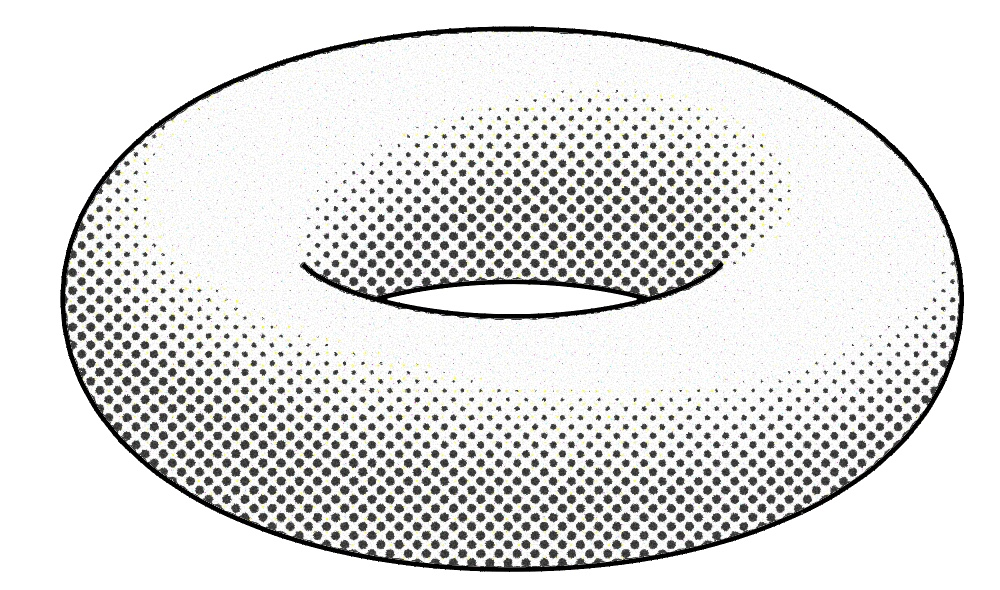
\includegraphics[scale=0.3]{graphics/diagrams/torus_non_vanishing_vector_field/result.jpg}
% 	\vspace{1em}
% 	\caption{A torus.}
% \end{figure}
%
% By relaxing our assumptions about the shape of space, geometry begins to quickly fill up with many such counter-intuitive non-Euclidean spaces and they find applications in unexpected places. Take for instance 
%
% \hspace{1em}
% % Many such axiomatic foundations exist, and lead 
%
% Let's start with the simple case of Euclidean space (think of a plane for instance) by describing some of its essential aspects. First and foremost Euclidean space is comprised of infinitely many points which \emph{extend continuously}, which informally means that Euclidean space is equipped with a qualitative concept of ``closeness''. Among other things, this 
%
% Euclidean space also comes with the stronger, quantitative notion of closeness -- this is known as \defn{distance}. A distance metric assigns to each pair of points a non-negative real number.

% \pagebreak

% \todo{The geometries they worked in were mostly flat, i.e. Euclidean and they relied on entirely (analytical?) methods to derive spatial relationships}
%
% \todo{Take a step back and see what data we have.}
%
% Classical geometry works in affine space, so we have: continuity of space, distance,  translation and homotethy. Translation gives us a global parallelism.
%
% Introduction of curvature
%
% Intrinstic  geometry via Theorema Egregium
%
% Symplectic manifolds, spin manifolds -> corresponding to physics
%
% Ehrlangen program

% At the scales they worked at, reality was best modelled by a plane or a (flat) three dimensional space.

% Homotopy classes of spaces
%
% PL manifolds
%
% During my last summer before graduating college, I went with some friends on a mountaineering trip up Banner peak, a picturesque mountain in the eastern Sierra Nevada range of California. 
% %
% % As we descended the glacier towards our base camp, ice axes in hand, I 
% So how \emph{do} we study objects which we can't touch, see, or possibly hope to visualize in their full complexity?
%
% There are two levels to understanding.
% \begin{enumerate}
% 	\item First, we
% \end{enumerate}
%
% Understanding an object by how it behaves with respect to other objects.
% \todo{spectral lines of atoms}
%
% One of the earliest methods to ``fingerprint'' topological objects was discovered by Euler.

% \cite{hatcher2002}


\chapter*{Conventions}\label{chap:conventions}
\addcontentsline{toc}{chapter}{Conventions}
\markboth{Conventions}{Conventions}
\chapter*{Conventions}

\subsection*{General}

\begin{itemize}
  \item Definitions of terms will be formatted {\color{blue}\emph{blue and emphasized}}, and hyperlinks will be formatted just blue (e.g. \cref{fig:first}).
  \item We use $\cong$ instead of $\oldcong$ to denote isomorphisms, diffeomorphisms, etc.
\end{itemize}

\subsection*{Algebra}

\begin{itemize}
  \item The group of units in a ring $A$ is denoted $A^\times$.
  \item A \defn{graded ring} is a ring $A$ equipped with a decomposition of its underlying group as $A=\bigoplus_{k\in \Z_{\geq 0}} A[k]$ such that the ring multiplication sends $A[k_1]\times R[k_2] \to A[k_1+k_2]$. Elements belonging to $A[k]$ are said to be \defn{homogeneous of degree $k$}[homogeneous element of a graded ring]. 
  \item A graded ring is said to be \defn{graded-commutative} if for any homogeneous elements $x\in A[k_1]$ and $y\in A[k_2]$, we have
    \[
      x\cdot y = (-1)^{k_1k_2} y\cdot x
    \]
  \item The \defn{completion}[completion of a graded ring] of a graded ring $A$ is the direct product $\widehat{A} = \prod_{k\geq 0} A[k]$.
  \item When expanding an element $a$ in a graded ring or completion of a graded ring as an infinite series, we use the notation
  \[
      a = a_0 + a_1t+a_2t^2+\cdots
  \]
  The variable $t$ should be understood as a notational formal variable.
  \item $A_{(1)}\subset A^\times$ denotes the units with monic leading coefficient (i.e. $a_0=1$).
\end{itemize}

\subsection*{Differential Topology}
\begin{itemize}
  \item A \defn{topological manifold} $M$ is a locally Euclidean second-countable Hausdorff space. \todo{boundary}
  \item A \defn{smooth structure} $\mathscr{S}$ on a topological manifold $M$ is a collection of open charts $\mathscr{S}=\{(U_\alpha, \varphi_\alpha)\}_{\alpha\in I}$ such that the transition functions 
	\begin{equation}\label{eq:transition-function}
		\lkxfunc{g_{\alpha\beta}}{\varphi(U_\alpha\cap U_\beta)}{\R^n\textrm{ or } \R^{n-1}\times [0,\infty)}
	\end{equation}
	are smooth for all $\alpha,\beta\in I$. We require that $\mathscr{S}$ be maximal with respect to this property, i.e. the addition of any chart $(U,\varphi)$ not in $\mathscr{S}$ breaks the smoothness of \cref{eq:transition-function}.
  \item Unless otherwise specified, all manifolds are assumed to be smooth, connected, and possibly with boundary. A \defn{closed}[closed manifold] manifold is a compact manifold with empty boundary.
  \item When introducing a manifold, we often put its dimension as a superscript. For example, ``let $M^n$ be a manifold'' should be read as ``let $M$ be an $n$-dimensional manifold''.

  \item We assume that all submanifolds $N\subset M$ are properly embedded and neat, i.e.
    \vspace{-0.5em}
    \begin{itemize}
      \item the inclusion $\iota : N \to M$ is a proper map,
      \item $\partial N\subset \partial M$,
      \item the boundary $\partial N$ intersects $\partial M$ transversally.
    \end{itemize}
\end{itemize}

\subsection*{Algebraic Topology}
\begin{itemize}
  \item Given a coefficient ring $R$, $\H^i(-; R)$ denotes the singular cohomology with coefficients in $R$, and $\H_i(-;R)$ denotes singular homology with coefficients in $R$. $\H^\bullet(-;R)$ is the singular cohomology ring.
  \item $\HdR$ denotes de-Rham cohomology, and $\Hc$ denotes compactly-supported de-Rham cohomology.
  \item Whenever we refer to a general (co)homology theory $h$, we mean one of the pairs:
    \begin{itemize}
      \item Singular (co)homology with coefficients in $R=\Z, \Z/2, \Z[1/2],$ or $\Q$.
      \item Compactly supported de-Rham cohomology and de-Rham cohomology.
    \end{itemize}
    The homology groups are denoted $h_i(-)$ and the cohomology groups are denoted $h_i(-)$. Note that all pairs 
\end{itemize}

\subsection*{Differential Geometry}
\begin{itemize}
  \item Vector bundles are over a field $\F=\R$ or $\C$, by default assumed to be $\R$.

  \item By default, we denote the total space of a vector bundle with normal math font, i.e. $E \to X$, and denote the bundle itself with calligraphic font, i.e. $\mathcal{E} : E \to X$. 

  \item The tangent bundle of a manifold $M$ is dented $\TT M$, with total space $\T M$.

  \item As with manifolds, a superscript $\mathcal{E}^k$ on a vector bundle denotes its rank. 

  \item Given a Riemannian inner product structure $\langle-,-\rangle$ on a vector bundle $\mathcal{E}^k$, we let $\S(\mathcal{E})$ be the associated sphere bundle (with fibers $S^{k-1}$) and $\D(\mathcal{E})$ the associated disk bundle (with fibers $D^k$). The total spaces of these bundles are
  \[
    \S(E) = \{ \xi\in E \mid \langle \xi, \xi\rangle =1 \}
    \quad\textrm{and}\quad
    \D(E) = \{ \xi\in E \mid \langle \xi, \xi\rangle\leq 1 \}
  \]
  respectively. Note that $\partial \D(E) = \S(E)$ as manifolds.
\end{itemize}


\chapter{Introduction}\label{chap:introduction}
% \begin{flushleft}
% 	\textsl{There is geometry in the humming of the strings,}\\
% 	\textsl{and there is music in the spacing of the spheres.}\\
% 	\rule[0pt]{21em}{0.5pt}\\
% 	-- \textsc{Pythagoras}\\
% 	\vspace{2em}
% \end{flushleft}

\begin{flushleft}
	\textsl{God created the integers,}\\
	\textsl{the rest is the work of man.}\\
	\rule[0pt]{13em}{0.5pt}\\
	-- \textsc{Leopold Kronecker}\\
	\vspace{2em}
\end{flushleft}

\todo{introduce, motivate, provide historical context.}

\begin{conjecture}[Poincar\'e Conjecture]
	Every closed topological $3$-manifold which is simply connected is homeomorphic to the $3$-sphere $S^3$.
\end{conjecture}

\begin{definition}
	If $U\subset \R^n$ is an open subset, a function $f : U \to \R^m$ is said to be \defn{smooth}[smooth function] if all partial derivatives of $f$ exist to all orders.
\end{definition}

\begin{definition}
	A \defn{smooth structure} $\mathscr{S}$ on a topological manifold $M$ (possibly with boundary) is a collection of charts $\mathscr{S}=\{(U_\alpha, \varphi_\alpha)\}_{\alpha\in I}$ such that the transition functions
	\begin{equation}\label{eq:transition-function}
		\lkxfunc{\varphi_\alpha\varphi_\beta^{-1}}{\varphi(U_\alpha\cap U_\beta)}{\R^n\textrm{ or } \R^{n-1}\times [0,\infty)}
	\end{equation}
	are smooth for all $\alpha,\beta\in I$. We require that $\mathscr{S}$ be maximal with respect to this property, i.e. the addition of any chart $(U,\varphi)$ not in $\mathscr{S}$ breaks the smoothness of \cref{eq:transition-function}.
\end{definition}
% A smooth structure gives rise to tangent spaces -- at each point of the3manifold there is a notion of infinitesimal direction, and the set of all such infinitesimal directions forms a vector space of tangent vectors. \todo{physics}

While the class of smooth manifolds offers a tempting for context for the exploration of the shape of space, it is far from the only type of manifold one can define. Another equally valid category in which to study topology of manifolds is $\Pl$, or the piecewise linear category. A $\Pl$ structure on a manifold consists of

\begin{conjecture}[Generalized Poincar\'e Conjecture]
	Letting $\mathscr{C}$ be either $\Top$, $\Pl$, or $\Diff$, any $\mathscr{C}$-manifold which is homotopy equivalent to the $n$-sphere $S^n$ is also $\mathscr{C}$-isomorphic to $S^n$.
\end{conjecture}

\begin{conjecture}[Hauptvermutung]
	\todo{this}
\end{conjecture}

\todo{questions about equivalence of TOP, PL, and DIFF}

\todo{goal of this chapter is provide some fundamental concepts needed to begin working on the problem}

\subsection{Morse Theory}

While a fully comprehensive introduction to Morse theory is outside of the scope of this thesis, we'll include a basic overview for completeness. A great classical introduction to Morse theory can be found in Milnor's book on the subject \cite{milnor1963morse}.

If $f : M \to \R$ is a smooth function on a manifold $M$, the points $p\in M$ where the differential $df_p : \T_p M \to \T_{f(p)} \R = \R$ vanish are known as \defn{critical points}, and their images in $\R$ are called \defn{critical values}. In terms of local coordinates $\{x^1,\ldots, x^n\}$ at $p$, this means that
\[
	\frac{\partial f}{\partial x^1}=\cdots=\frac{\partial f}{\partial x^n} = 0.
\]
A critical point $p\in M$ is said to be \defn{non-degenerate}[non-degenerate point] if the matrix
\[
	\everymath={\displaystyle}
	\renewcommand*{\arraystretch}{2}
	H_f(p) = \begin{pmatrix}
		\frac{\partial^2 f}{\partial x^1\partial x^1} & \cdots &
		\frac{\partial^2 f}{\partial x^1\partial x^n}                   \\
		\vdots                                        & \ddots & \vdots \\
		\frac{\partial^2 f}{\partial x^n\partial x^1} & \cdots &
		\frac{\partial^2 f}{\partial x^n\partial x^n}                   \\
	\end{pmatrix}(p)
\]
is invertible at $p$. This is called the \defn{Hessian matrix} of $f$ at $p$, and in this formulation depends on our chosen coordinate system.
There is a coordinate independent way to define the Hessian as a symmetric bilinear form on $\T_p M$ which makes the coordinate invariance of the condition of non-degeneracy manifestly apparent.

\begin{definition}
	The \defn{index}[index of a function] of $f$ at a point $p$ is the maximal dimension of a subspace on which $H_f(p)$ is negative definite, i.e. it is the dimension of $\{v\in \R^n \mid v^\intercal H_f(p) v < 0\}.$
\end{definition}

The index of a function at a point essentially describes the ``shape'' of the function out of a list of finitely many possible shapes. Remember, the index of a function on an $n$-dimensional manifold must be an integer between $0$ and $n$. For instance, in the case of a surface there are three possible shapes -- when both coordinates curve up we get a bowl facing up, when one curves up and one curves down we get a saddle, and when both coordinates curve down we get a bowl facing down. These shapes correspond to indices of $0$, $1$, and $2$ respectively.
\begin{figure}[ht]
	\centering
	\todo{draw figure}
	\medskip
	\caption{An upward bowl, saddle, and downward bowl.}
\end{figure}

The fundamental lemma of Morse theory makes rigorous this notion of a manifold having a shape dictated by a real-valued function -- there is always a local coordinate system which puts the function into a standard form depending on the index.

\begin{lemma}[Morse Lemma]\label{lemma:morse}
	Let $p$ be a non-degenerate critical point of $f$. There is a local coordinate system $(y^1,\ldots, y^n)$ at $p$ such that
	\[
		f(y^1,\ldots, y^n)=f(0)-\left[(y^1)^2 + \cdots + (y^{\ell})^2\right] + \left[(y^{\ell + 1})^2 + \cdots + (y^n)^2\right].
	\]
	where $\ell$ is the index of $f$ at $p$.
\end{lemma}
\begin{proof}
	Let's assume without loss of generality that $f(p)=0$. Given any local coordinate system $(x^1,\ldots, x^n)$ at $p$, we can write
	\[
		f(x^1,\ldots, x^n) = \sum_{1\leq j \leq n} x^j g_j(x^1,\ldots, x^n)
	\]
	where $g_j$ are functions satisfying $g_j(0)=(\partial f / \partial x^j)(0)$. 
	This can be achieved by setting $g_j(x_1,\ldots, x_n) = \int_0^1 (\partial f/\partial x^j)(tx_1, \ldots, tx_n)\,dt$. Since $p$ is a critical point

	\todo{basic idea}
\end{proof}

Inspired by this lemma, we might call a function $f : M \to \R$ a \defn{Morse function} if all critical points are non-degenerate.

\begin{corollary}
	Non-degenerate critical points are isolated.
\end{corollary}

For a brief demonstration of the power of the Morse lemma, we'll prove Reeb's theorem, a Morse theoretic criterion for a compact manifold to be homeomorphic to a sphere. Throughout the thesis, we'll usually defer to the more powerful $h$-cobordism theorem to prove that a manifold is homoemorphic to a sphere. However, it is useful to not always rush for the flamethrower when trying to kill a fly -- a simple swatter might do the trick. We'll see a direct application of this lighter theorem in \cref{sec:first-exotic-sphere}.

\begin{theorem}[Reeb]\label{thm:reeb}
	If $M$ is a compact manifold and $f$ is a Morse function with exactly $2$ critical points, then $M$ is homeomorphic to a sphere.
\end{theorem}
\begin{proof}
	Firstly, by compactness of $M$ we can find a global minimum $f(x_0)$ and global maximum $f(x_1)$ for some distinct points $x_0$ and $x_1$ (otherwise the function would be constant and not a Morse function with $2$ critical points). We can normalize the function $f$ to have $f(x_0)=0$ and $f(x_1)=1$ without loss of generality. It follows that $x_0$ is a non-degenerate critical point of index 0 and $x_1$ is a non-degenerate critical point of index $n$.
	By the Morse lemma (\ref{lemma:morse}), there is a neighborhood $x_0\in U_0$ with local coordinates $\{y^1,\ldots, y^n\}$ such that 
	\[
			f(y^1,\ldots, y^n) = (y^1)^2 + \cdots + (y^n)^2.
	\]
	This gives a Riemannian metric $(dy^1)^2+\cdots+(dy^n)^2$ on $U$ which can be extended to all of $M$ by partitions of unity.
	% A Riemannian metric on a manifold $M$ determines an isomorphism $\T^\d M \cong \T M$, and hence an isomorphism $\Omega^1(M)=\Gamma(\T^\d M) \cong \Gamma(\T M)=\X(M)$ between the space of $1$-forms and the space of vector fields. Composing this isomorphism with the exterior derivative $d : \Omega^0(M)\to \Omega^1(M)$ gives the gradient operator $\nabla : \Omega^0(M) \to \X(M)$ sending a function to its vector field. 

	Given a Riemmanian structure, there is a gradient operator $\nabla : \Omega^0 \to \X(M)$ sending functions to vector fields.
	In our case, the vector field $\nabla f$ is non-zero everywhere except for at $x_0$ and $x_1$. We thus have a normalized vector field $\nabla f/\|\nabla f\|^2$
	defined everywhere except for at $x_0$ and $x_1$. Let $\varphi_t : M \to M$ be the global flow corresponding to this vector field, i.e. the unique solution to the differential equation
	\[
	\left.\frac{d\varphi_t(p)}{dt}\right|_{t=0} = \frac{\nabla f(p)}{\|\nabla f(p)\|^2}
	\]
	for all $p\in M\setminus \{x_0,x_1\}$. By the chain rule, it follows that
	\[
		\frac{d(f\circ \varphi_t(p))}{dt}=\left\langle \frac{d\varphi_t(p)}{dt}, \nabla f\right\rangle = \left\langle \frac{\nabla f}{\|\nabla f\|^2}, \nabla f\right\rangle=1.
	\]
	In particular, this implies that $f\circ \varphi_t(p) = f(p)+t$. 

	\todo{finish the proof}
\end{proof}

The basic ideas used in the proof of Reeb's theorem can be radically generalized.

\begin{definition}
	For any $a\in \R$, the \defn{level set} of a smooth function $f : M \to \R$ is the set 
	\[
		M_a = f^{-1}(-\infty, a] = \{ p\in M \mid f(p)\leq a)\}.
	\]
\end{definition}

\begin{figure}
\end{figure}

\begin{theorem}
	Let $f : M \to \R$ be a smooth function and suppose $f^{-1}[a,b]$ contains no critical points of $f$ for real numbers $a<b$. Then $M_a$ is diffeomorphic to $M_b$. Furthermore $M_a$ is a deformation retract of $M_b$.
\end{theorem}

\begin{theorem}
	Let $f : M \to \R$ be a smooth function and let $p$ be a non-degenerate critical point of index $\ell$. Letting $c=f(p)$, suppose that $f^{-1}[c-\epsilon, c+\epsilon]$ is compact and contains no critical points of $f$ aside from $p$. For sufficiently small $\epsilon$, the level set $M^{c+\epsilon}$ has the homotopy type of $M^{c-\epsilon}$ with an $\ell$-cell attached.
\end{theorem}

\begin{theorem}
	If $f$ is a Morse function with compact level sets (for instance if $M$ is compact), then $M$ has the homotopy type of a CW-complex with a cell in each dimension $\ell$ for each critical point of index $\ell$.
\end{theorem}

\todo{finish}

\subsection{Cobordism}\label{sec:cobordism}

The basic principle of cobordism is to declare two manifolds equivalent if there is a manifold a dimension higher which connects the two manifolds. As an equivalence relation, cobordism is generally far looser than the notions of homoemorphism or diffeomorphism. In most dimensions, classifying manifolds up to strict notions of homeomorphism or diffeomorphism is provably impossible -- from a computational complexity standpoint such problems are undecidable. Cobordism on the other hand is loose enough to allow for a full classification.

\begin{remark}
	Note that the implied compactness assumption throughout the thesis is important here, otherwise any manifold $M$ is trivially the boundary of $M\times [0,\infty)$. 
\end{remark}

\begin{definition}
	An \defn{unoriented cobordism} between closed $n$-manifolds $M_1$ and $M_2$ is an $(n+1)$-manifold $W$ with $\partial W = M_1\sqcup M_2$. We use the notation $W : M_1\bord M_2$ to refer to the cobordism.
\end{definition}

\begin{definition}
	An \defn{oriented cobordism} between closed oriented $n$-manifolds $M_1$ and $M_2$ is an oriented $(n+1)$-manifold $W$ with $\partial W = M_1\sqcup (-M_2)$. We use the notation $W : M_1\sobord M_2$ to refer to the cobordism.
\end{definition}

\begin{example}
	Within some category of 
\end{example}

\begin{figure}[ht]
	\centering
	\import{graphics/temp-diagrams/}{pair-of-pants.pdf_tex}
	\caption{A cobordism $W$ between $S^1$ and $(S^1\sqcup S^1)$.}\label{fig:pair-of-pants}
\end{figure}

For a simple example of a cobordism between a circle and a disjoint union of circles, see \cref{fig:pair-of-pants}. Note that this cobordism could be made much simpler by removing the handle. Simplifying cobordisms in this way is one of the major applications

\begin{definition}
	The \defn{$\bm{k}$-th oriented cobordism group}[oriented cobordism group] $\Omega^\SO_k$ is the abelian group of oriented cobordism classes of closed $k$-manifolds\footnote{We do not require manifolds to be connected in this definition.}
	under disjoint union. The identity component is the empty set $\varnothing$, and negation is given by reversing orientation. Similarly, the \defn{$k$-th unoriented cobordism group}[unoriented cobordism group] $\Omega_k$ is the abelian group of cobordism classes of closed $k$-manifolds under disjoint union.
\end{definition}

Note that the oriented cobordism group can be thought of as a $\Z$-module, with multiplication action on a closed manifold $M$ given by
\[
	n \cdot M = \begin{cases} M\sqcup \cdots \sqcup M & n > 0,\\ (-M)\sqcup \cdots \sqcup (-M) & n < 0,\\ \emptyset & n=0,\end{cases}
\]
for all $n\in \Z$, where $\sqcup$ is repeated $|n|$ times. Since there is no notion of negation in the unoriented case, the unoriented cobordism group is a $\Z/2$-module.

\begin{example}
	There is an isomorphism $\Omega_0\cong \Z/2$. An unoriented 0-dimensional manifold is just a set of points. Any pair of points is cobordant to the empty set by a path connecting them. Since adding pairs of points doesn't change the cobordism type, the number of points modulo 2 determines the cobordism class entirely.
\end{example}

\begin{example}
	There is an isomorphism $\Omega_0^\SO \cong \Z$. An oriented 0-dimensional manifold is still a set of points, however the orientation now equips each point with a ``charge'', we might label them as $+$ or $-$. Note that points of opposite ``charges'' cancel out by a path between them oriented from $-$ to $+$. Given some set of points of various charges, we can always eliminate pairs of opposite charges and are left with a homogeneous set of charge. Adding up all of the pluses or minuses, we get an integer. This integer determines the cobordism class, and is invariant to adding or removing pairs of opposing charge.
\end{example}

\begin{example}
	Both the oriented and unoriented cobordism groups are trivial in dimension 1, since every circle is the boundary of a disk.
\end{example}

In higher dimensions, the classification becomes much more interesting. 

\begin{figure}[ht]
	\renewcommand{\arraystretch}{1.2}
	\centering
	\begin{tabular}{r||c|c||c|c}
		$k$ & $\Omega_k$ & generators & $\Omega_k^\SO$ & generators \\
		\hline
		$0$ & $\Z/2$ & a point & $\Z$ & a point\\
		$1$ & $0$ & & $0$ & \\
		$2$ & $\Z/2$ & $\RP^2$ & $0$ & \\
		$3$ & $0$ & & $0$ & \\
		$4$ & $\Z/2\oplus \Z/2$ & $\RP^4$, $\RP^2\times \RP^2$ & $\Z$ & $\CP^2$ \\
		$5$ & $\Z/2$ & $\SU_3/\SO_3$ & $\Z/2$ & $\SU_3/\SO_3$\\
		$6$ & $(\Z/2)^{\oplus 3}$ & $\RP^6$, $\RP^2\times \RP^4$, $(\RP^2)^{\times 3}$, & $0$ & \\ 
		$7$ & $\Z/2$ & $(\SU_3/\SO_3) \times \RP^2$ & $0$ & \\ 
		$8$ & $(\Z/2)^{\oplus 4}$ & $\RP^8, \RP^6\times \RP^2, \cdots$ & $\Z\oplus \Z$ & $\CP^4, \CP^2\times \CP^2$\\
	\end{tabular}
	\medskip
	\caption{Structure of unoriented and oriented cobordism groups.}\label{fig:cobordism-structure-table}
\end{figure}

The structure of \cref{fig:cobordism-structure-table} makes a lot more sense in the context of 

\begin{proposition}
	The product of manifolds is a well-defined operation with respect to cobordism.
\end{proposition}
\begin{proof}
	\todo{proof}
\end{proof}

\begin{definition}
	The \defn{oriented cobordism ring} $\Omega^\SO_\bullet$ is the set of oriented cobordism classes of closed manifolds under the operations of disjoint union and product.
\end{definition}

The oriented cobordism ring has a grading by
\[
	\Omega_\bullet^\SO = \bigoplus_{k\geq 0} \Omega^\SO_k.
\]

\todo{finish this section, cobordism with additional structure}

\todo{Ren\'e thom cobordism ring determination, will be used later in hirzebruch}

\begin{remark}
	There are several generalizations of the notion of cobordism.\todo{cobordism ring with structure, link to framed cobordism}
\end{remark}


\subsection{The $h$-Cobordism Theorem}

\begin{definition}
	A cobordism $W : M_1\bord M_2$ is said to be an \defn{$\bm{h}$-cobordism} if $M_1$ and $M_2$ admit deformation retracts from $W$. We denote $h$-cobordisms by $\hbord$ when the category of manifolds is clear.
\end{definition}

If $M_1$ and $M_2$ are $h$-cobordant, then clearly they have the same homotopy type since they are deformation retracts of the same space.

\begin{theorem}[$h$-cobordism]\label{thm:h-cobordism}
	Within some category of manifolds $\mathscr{C}$, if $M$ and $N$ are closed, simply-connected manifolds of dimensions $\geq 5$ and $W : M \hbord N$ is a simply-connected $h$-cobordism, then $W$ is $\mathscr{C}$-isomorphic to the cylinder $M\times [0,1]$. Furthermore, the isomorphism can be chosen to be the identity on $M\times \{0\}$.
\end{theorem}
\begin{proof}
	As with Morse theory, a proof of the $h$-cobordism theorem could easily fill up an entire thesis so we'll only briefly summarize the proof here.

	\todo{talk about handlebodies}
\end{proof}

\begin{theorem}
	In the manifold categories $\Top$ and $\Pl$, the generalized Poincar\'e conjecture is true in dimensions $\geq 5$.
\end{theorem}
\begin{proof}
	\todo{cone construction, fails for $\Diff$ because you can't take a smooth cone.}
	\todo{mention method of engulfing?}
\end{proof}

\todo{why this argument fails for $\Diff$}

\begin{corollary}\label{thm:h-cobordism-diffeomorphism}
	In the smooth oriented manifold category, two simply-connected closed manifolds of dimensions $\geq 5$ are $h$-cobordant if and only if they are diffeomorphic (by an orientation preserving diffeomorphism).
\end{corollary}
\begin{proof}
	If $f : M_1 \to M_2$ is a diffeomorphism between manifolds $M_1$ and $M_2$, they are $h$-cobordant by the manifold $W=M_1\times [0,1]\cup_f M_2$, where we glue $M_2$ onto $M_1\times \{1\}$ in $M_1\times [0,1]$ by $f$.
	Conversely, if $W : M_1\sohbord M_2$ is an $h$-cobordism, by the $h$-cobordism theorem (\ref{thm:h-cobordism}) there must be a diffeomorphism $f : W \to M_2$ must map to $M_1\times \{1\}$, this gives a diffeomorphism $M_2 \to M_1$. If we choose $f$ to reverse orientation on $M_1\to M_1\times \{0\}$, then the restriction $f|_{M_2}$ will preserve orientation.
\end{proof}

We've thus arrived at our first major simplification to the problem of classifying exotic spheres in dimensions $\geq 5$ -- in order to classify smooth structures, it's enough to classify the $h$-cobordism classes of smooth manifolds which are topological spheres, and to find smooth manifolds which are topological spheres it suffices to consider smooth manifolds which have the homotopy type of a sphere.

\begin{definition}
	A \defn{homotopy $\bm{n}$-sphere}[homotopy sphere] is a smooth manifold which is homotopy equivalent to the sphere $S^n$.
\end{definition}

\begin{definition}
	We use the notation $\Theta^n$ to refer to the pointed set of $h$-cobordism classes of homotopy $n$-spheres (the basepoint is the ordinary sphere $S^n$).
\end{definition}

\subsection{Groups of Homotopy Spheres}

The last ingredient in our setup of the classification of exotic spheres is a group structure on the set of homotopy spheres.
The simplest additive structure between topological spaces is a disjoint union, and this is the group operation used in cobordism. A problem with the disjoint union is that it results in disconnected spaces. If the spaces involved are manifolds of the same dimension, there is a connected version of a disjoint union -- we can glue the manifolds together by a ``tube''.

\begin{definition}
	Let $M_1$ and $M_2$ be oriented smooth $n$-dimensional manifolds. Choose embeddings of $n$-dimensional disks $\iota_1 : D^n \to M_1$ and $\iota_2 : D^n \to M_2$ such that $\iota_1$ preserves orientation and $\iota_2$ reverses it. The \defn{connected sum} of $M_1$ and $M_2$, denoted $M_1\+ M_2$, is the space
	\[
		M_1\+M_2 = (M_1 \setminus \iota_1(0))\cup_g (M_2 \setminus \iota_2(0))
	\]
	where $g$ identifies $\iota_1(tu)$ with $\iota_2((1-t)u)$ for each unit vector $u\in \partial D^n$ and $t\in (0,1)$. We choose an orientation for $M_1\+ M_2$ which is compatible with the orientation of $M_1$ and $M_2$, and this works because $g$ is orientation preserving.
\end{definition}

\begin{figure}[ht]
	\centering
	\import{graphics/temp-diagrams/}{connected-sum.pdf_tex}
	\caption{Construction of the connected sum.}\label{fig:connected-sum}
\end{figure}

Proving that the connected sum operation is well-defined in the smooth category takes more work than one might expect. For brevity, we'll defer to a technical result by Palais.

\begin{theorem}[Disk Theorem]
	If $M$ is an oriented smooth $n$-dimensional manifold and we have orientation preserving disk embeddings $\iota_1,\iota_2 : D^n \to M$, then there is a diffeomorphism $f : M \to M$ such that $\iota_1 = f\circ \iota_2$.
\end{theorem}
\begin{proof}
	See Theorem~B in \cite{palais1960extending}.
\end{proof}

\begin{corollary}
		The connected sum is well-defined, associative, and commutative up to orientation preserving diffeomorphism.
\end{corollary}

\begin{theorem}
	The connected sum turns $\Theta^n$ into a group with identity element $S^n$.
\end{theorem}
\begin{proof}
	\todo{write the proof}

	\begin{changemargins}
	\begin{lemma}
		Let $M_1, M_1'$ and $M_2, M_2'$ be closed simply-connected manifolds. If $M_1\sohbord M_1'$ and $M_2\sohbord M_2'$ are $h$-cobordant, then there is an $h$-cobordism $(M_1\+ M_2) \sohbord (M_1'\+M_2')$.
	\end{lemma}
	\begin{proof}
	\todo{write the proof}
	\end{proof}
	\end{changemargins}

	\begin{changemargins}
	\begin{lemma}
		A simply-connected manifold $M$ is $h$-cobordant to $S^n$ if and only if $M$ bounds a contractible manifold.
	\end{lemma}
	\begin{proof}
	\todo{write the proof}
	\end{proof}
	\end{changemargins}

	\noindent This completes the proof.
\end{proof}

The terminology of algebra now open up to us. In the time since 

\subsection{Twisted Spheres}
	The following section should be read as an extended remark on the definition of connected sum, as we will not use any of the following results in the rest of the thesis.

	The definition of connected sum for smooth manifolds is slightly stronger than the definition for topological manifolds. In the topological category, we could simply cut out open disks from both manifolds and identify their boundaries, i.e. we set
	\begin{equation}\label{eq:connected-sum-in-topological-category}
		M_1\# M_2 = (M_1\setminus \Int(\iota_1(D^n)))\cup_g (M_2\setminus \Int(\iota_2(D^n)))
	\end{equation}
	where $g : \partial \iota_1(D^n) \to \partial \iota_2(D^n)$ is any orientation-reversing homeomorphism. This definition turns out to be well-defined in the topological category, although proving this takes a considerable amount of work. \todo{cite}

	However, the connected sum in the topological category will not give a unique connected sum in the smooth category, in fact far from it. Interestingly enough, the failure for \cref{eq:connected-sum-in-topological-category} to give a unique smooth manifold is related to exotic spheres in the following way. Whenever we have an orientation-preserving diffeomorphism $f: S^{n-1}\to S^{n-1}$, identifying $\partial D^n = S^{n-1}$ allows us to glue together disks to get $T(f)=D^n\cup_f D^n$. This is a smooth manifold which is the (topological) connected sum of two spheres so must be homoemorphic to a sphere. The manifolds $T(f)$ are called \defn{twisted spheres} since they are built by ``twisting together'' two disks by $f$. 

	We can interpret the twisted sphere construction as a map $T: \op{Diff}^+(S^{n-1})\to \Theta^n$ sending an orientation-preserving diffeomorphism $f : S^{n-1} \to S^{n-1}$ to the twisted sphere $T(f)$. For any (smooth) path $\omega : I \to \op{Diff}^+(S^{n-1})$, we can build an $h$-cobordism 
	\[ (D^n\times I)\cup_\omega (D^n\times I) : T(\omega_0) \sohbord T(\omega_1)\]
	where we interpret the path $\omega$ as a smooth homotopy $\omega : I\times S^{n-1}\to\S^{n-1}$ between diffeomorphisms $\omega_0, \omega_1 : S^{n-1} \to S^{n-1}$. For $n\geq 5$, \cref{thm:h-cobordism-diffeomorphism} implies that $T(\omega_0)$ is diffeomorphic to $T(\omega_1)$ so the map $T$ only depends on the path component of $f\in \op{Diff}^+(S^{n-1})$.
	Next, note we can extend $f$ to a diffeomorphism on the interior of the disk, the resulting twisted sphere must be diffeomorphic to a sphere. By a similar argument, we can reduce to path-components. Altogether, we have an exact sequence (of sets)
	\begin{equation}\label{eq:twisted-sphere-exact-sequence-proto}
		\pi_0 [\op{Diff}^+(D^n)] \lkxto \pi_0 [\op{Diff}^+(S^{n-1})] \lkxto[T] \Theta^n.
	\end{equation}
	Finally, if we take any homotopy sphere $\Sigma\in \Theta^n$, cutting out the interiors of any embedded open disks $D_1, D_2\subset \Sigma$ gives an $h$-cobordism $\Sigma\setminus(D_1\cup D_2) : \partial D_1 \sohbord \partial D_2$. If $n\geq 6$, the $h$-cobordism theorem (\ref{thm:h-cobordism}) implies that $\Sigma \setminus (D_1\cup D_2)$ is diffeomorphic to a cylinder $\partial D_2\times [0,1]$. It follows that $\Sigma$ is a twisted sphere corresponding to the diffeomorphism $\partial D_1 \cong \partial D_2$ coming from the $h$-cobordism.
	When $n\geq 6$, the exact sequence \cref{eq:twisted-sphere-exact-sequence-proto} therefore extends to 
	\[
		\pi_0 [\op{Diff}^+(D^n)] \lkxto \pi_0 [\op{Diff}^+(S^{n-1})] \lkxto[T] \Theta^n \lkxto 0.
	\]
	In 1970, Cerf proved the pseudoisotopy theorem \cite{cerf1970pseudoisotopy}, one of the consequences of which implies that $\pi_0[\op{Diff}^+(D^n)]=0$ for $n\geq 6$. From this it follows that:

	\begin{proposition}
		For $n\geq 6$, we have a bijection $\Theta^n \cong \pi_0[\op{Diff}^+(S^{n-1})]$.
	\end{proposition}

	In my subjective opinion, this is the most canonical way to observe the phenomenon of exotic smooth structures on the spheres. Rather than work with a set of abstract smooth manifolds and diffeomorphisms between them, it's possible to interpret the set of smooth structures on a sphere as the set of path-components of diffeomorphisms on a specific sphere. This bijection is also a reason as to why some theoretical physicists care about exotic spheres. \todo{change of coordinates, 10-dimensional change of coordinates (with compact support) has 992 components.} 
	For instance, Witten's 1985 paper \cite{witten1985global} on global anomalies in string theoretic models of gravity contains extensive discussions on exotic spheres, and the use of geometric invariants in detecting them.

\subsection{The Poincar\'e Hypothesis in Low Dimensions}

The reduction of the problem of finding diffeomorphism classes of homotopy spheres to the problem of finding $h$-cobordism classes of spheres is a massive simplification, and allows for a complete general classification.
The lack of an $h$-cobordism theorem in dimensions $<5$ means that practically none of the techniques developed in this thesis will work for these low dimensions and so they must be analyzed manually. The uniqueness of smooth structure on a circle is a standard exercise in introductory topology. In dimension $2$, we can give the sphere a complex structure making it a Riemann surface, and by the uniformization theorem, the complex structure must be conformally equivalent to the Riemann sphere. This is the unique complex structure and so it has a unique smooth structure.

For the case of dimension $3$, the uniqueness of a smooth structure is a orders of magnitude harder to prove. In the 1950s, Moise proved the equivalence of topological, PL, and smooth structures for compact $3$-manifolds. These results are outlined in the book \cite{moise1977geometric}. For decades, the uniqueness of smooth structures on the 3-dimensional sphere was thus relegated to a proof of the topological Poincar\'e hypothesis in 3-dimensions -- the original conjecture proposed of Poincar\'e in 1904. The topological Poincar\'e hypothesis had already been proved in dimensions $\geq 5$ by Smale, Stallings, and Zeeman in the early 1960s, and in dimension $4$ by Freedman's 1982 classification \cite{freedman1982} of simply-connected topological $4$-manifolds using many of the techniques we'll discuss in this thesis. Yet, the stubborn third dimension remained.
This proof finally came in 2003 as a consequence of Perelman's proof of Thurston's geometrization conjecture, a general classification for 3-dimensional geometries.
The battle with $3$-manifolds was a tough one, and it took hundreds of pages of hard analysis and Riemannian geometry by Hamilton and Perelman.
The basic idea by Hamilton to prove the Poincar\'e conjecture involved giving a
closed $3$-manifold a Riemannian metric $g_{\mu\nu}$, and then evolving this metric in time $\lambda$ by a differential equation involving the Ricci curvature tensor
\begin{equation}
	\frac{\partial g_{\mu\nu}}{\partial \lambda} = -2\mathcal{R}_{\mu\nu}.
	% \hspace{-3em}\tag{Ricci Flow Equation}
\end{equation}
This is known as the Ricci flow equation, and it forces the metric to change in such a way as to make distances decrease in directions of positive curvature.
Ricci flow can be used to ``smooth out'' the curvature of a nice enough $3$-manifold until it has constant curvature. In particular, simply connected manifolds turn into spheres under this regime, proving the Poincar\'e hypothesis.
Unfortunately, singularities can form when solving the Ricci flow equations, and it takes a careful application of the ideas of surgery to get around them. Perelman proved that this ``Ricci flow with surgery'' was always possible, turning Hamilton's ambitious program into rigorous mathematical machinery. For a comprehensive introduction to Perelman and Hamilton's proof of the geometrization conjecture, see \cite{morgantian2007ricci}.

The last remaining case of the generalized Poincar\'e conjecture is the classification of smooth (and equivalently PL) structures on spheres in dimension $4$. It remains hopelessly unsolved as of the conclusion of this thesis in March 2025. There are some candidates

\todo{talk a bit more about this, exotic $\R^4$s and why people suspect there might be exotic spheres in dimension 4}


% \todo{define PL, Diff, Top etc, show differences for instance cone construction}
%
%
%
%
%
% \begin{definition}
%   A closed oriented (smooth) $n$-manifold $M$ is called a \defn{homotopy sphere} if it has the homotopy type of the $n$-sphere $S^n$. An \defn{exotic sphere} is a homotopy $n$-sphere which is not diffeomorphic to the standard $n$-sphere $S^n$.
% \end{definition}
%
% \subsection*{Why is this complicated?}
%
% Any homotopy sphere is \defn{stably parallelizable} -- meaning the stable isomorphism class of its tangent bundle is trivial.
%
% \begin{theorem}
%   If $\Sigma$ is a homotopy $n$-sphere, then $\T \Sigma \oplus \underline{\R}$ is trivial. 
% \end{theorem}
% \begin{proof}
% \end{proof}
%
% In fact, a much stronger result holds true.
% \begin{theorem}
%   If $\Sigma$ is a homotopy $n$-sphere with $f : S^n \to \Sigma$ the homotopy equivalence, then there is a bundle isomorphism $f^*\T\Sigma \approx \T S^n$.
% \end{theorem}
% \begin{proof}
% \end{proof}
%
% \subsection*{Groups of Homotopy Spheres}
%
% See \cite{milnor1963groups} and \cite{levine1985lectures}
%
% \begin{definition}
%   Let $\Theta^n$ denote the group of diffeomorphism classes homotopy $n$-spheres under the operation of connected sum.
% \end{definition}
%
% \begin{definition}
% \end{definition}
%
% \begin{definition}
%   Let $\bP_{n+1}$ denote the subgroup of $\Theta^n$ of (classes of) homotopy $n$-spheres which bound parallelizable manifolds.
% \end{definition}
%
% \begin{theorem}[Kervaire-Milnor]
%   The group of homotopy $(4k-1)$-spheres bounding parallelizable manifolds is a cyclic group of order:
%   \[
%     |\bP^{4k}| = 2^{2k-2}(2^{2k-1}-1)\varepsilon_k\cdot \mathrm{num}(B_{2k}/4k) 
%   \]
% \end{theorem}
%
% \subsection*{The Kirby-Siebenmann Class}
%
% \begin{theorem}
%   For $n\geq 5$, there is an isomorphism $\pi_n(\pl/\diff)\approx \Theta^n$.
% \end{theorem}
%
% \subsection*{Global Gravitational Anomalies}
%
% See \cite{witten1985global}.


\chapter{Fundamentals of Surgery Theory}\label{chap:construction}

\begin{flushleft}
	\textsl{}\\
	\rule[0pt]{15em}{0.5pt}\\
	\textsl{-- }
	\vspace{2em}
\end{flushleft}

Within seven years of Milnor's 1956 announcement \cite{milnor1956manifolds} of his discovery of an exotic smooth structure on the $7$-sphere, the smooth structures on spheres of all but some tricky dimensions were completely classified  -- at the very least the problem was reduced to several better understood problems (see \cite{milnor1960homotopyspheres} and \cite{milnor1963groups}).
Such a quick turnaround is uncommon in mathematics, and this period of rapid growth starting in the late 1950s up until the late 1970s has been referred to as the ``golden age of topology''.
One of the great discoveries which emerged from this flurry of research was \defn{surgery theory}, a collection of techniques used to alter the topology of a manifold in a controlled way. This is usually done with respect to a loose notion of equivalence like cobordism -- for instance, we might use surgery to construct the simplest representative of a particular cobordism class.

In \cref{chap:introduction}, we saw how the problem of constructing and classifying exotic spheres can be reduced to a problem in cobordism, at least in dimensions $\geq 5$. This reduction gives us a foothold into the seemingly intractible problem of classifying smooth structures on spheres, but the resulting cobordism problem is still very hard.
Part of the difficulty is the almost complete lack of geometric information on homotopy spheres. A homotopy-sphere is, by definition, homotopy equivalent to a sphere, and so most of our usual invariants don't give us any useful information. However, there is a clever remedy to this issue. A useful principle in geometric topology is that the structure of manifolds is tightly coupled to the structure of manifolds which they bound.  The idea of studying $n$-dimensional topology by means of $(n+1)$-dimension topology with boundary is ubiquitous across mathematics and physics. \todo{mention cobordism, geometric invariants in later section, chern-simons theory}

\begin{definition}
	A manifold $W$ with boundary $X$ is said to be a \defn{coboundary} of $X$.
\end{definition}

Up to homeomorphism, a homotopy $n$-sphere $\Sigma$ always has a topological coboundary. For instance, we can take the disk $D^{n+1}$ and glue $\Sigma$ to $\partial D^{n+1}$. 
However, for any non-trivial homotopy sphere which \emph{does} have a smooth coboundary,\footnote{Not all homotopy spheres have a smooth coboundary -- we study these spheres in \cref{chap:homotopy}.} the topology of the coboundary can't be contractible like in the case of the disk, otherwise the homotopy sphere would be trivial by the $h$-cobordism theorem. In other words, by lifting to a coboundary, the diffeomorphism type of the boundary becomes dependent on the \emph{homotopy} type of the coboundary. 

It's much easier to study manifolds up to homotopy type, so we'll begin our exploration of $\Theta^n$ by considering those homotopy spheres which have a (smooth) coboundary. To make the study of the coboundary even simpler, we'll require this coboundary to be parallelizable.
\begin{definition}
	A manifold $M$ is said to be \defn{parallelizable}[parallelizable] if there exists a trivialization of its tangent bundle $\T M$.
\end{definition}
The condition of parallelizability turns out to be an immensely useful constraint to impose on a coboundary -- it's not too strict as to cause all topological invariants to vanish, but still simplifies many results. For instance, we'll see in \cref{chap:detection} how the vanishing of characteristic classes for a parallizable coboundary helps us construct simple and workable geometric invariants for homotopy spheres.

\begin{definition}
	Let $\bP^{n+1}\subset \Theta^n$ be the set of homotopy spheres with a parallelizable coboundary.\footnote{It's possible to interpret this inclusion as a boundary map $b : P^{n+1} \to \Theta^n$ in a long exact sequence. We'll see this perspective in \cref{sec:kervaire-milnor-braid}.}
\end{definition}

It's fairly clear that the condition of having a parallelizable coboundary is invariant under $h$-cobordism -- whenever $\Sigma_1\sohbord \Sigma_2$, a coboundary $W$ of $\Sigma_1$ can be used to construct a coboundary $W\cup_f \Sigma_2$ of $\Sigma_2$, where $f : \Sigma_1 \to \Sigma_2$ is a diffeomorphism corresponding to the $h$-cobordism. Checking that the group operation of connected sum preserves parallelizability of a coboundary is less clear. Since the connected sum is only defined on the base manifolds, it's useful to extend the operation to the coboundaries the manifolds being summed.

Let's define the half-disk $D_h^{n+1}$ by
\[
	D_h^{n+1} = \{ (x_1,x_2,\ldots, x_{n+1})\in\R^{n+1} \mid |x|\leq 1, x_1\geq 0\}
\]
and embedded the $n$-disk $D^n\subset D_h^{n+1}$ by setting $x_1=0$. Note that $\partial D_h^{n+1}= D^n$.
\begin{definition}
	Let $W_1$ and $W_2$ be oriented smooth $(n+1)$-dimensional manifolds with connected boundary. Choose embeddings of pairs $\iota_i : (D_h^{n+1},D^n)  \to (W_1,\partial W_1)$ and $\iota_2 : (D_h^{n+1}, D^n) \to (W_2, \partial W_2)$ such that $\iota_1$ preserves orientation and $\iota_2$ reverses it. The \defn{connected sum along the boundary} is defined to be the glueing
	\[
		(W_1,\partial W_1)\+(W_2,\partial W_2) = (W_1\setminus \iota_1(0))\cup_g (W_2\setminus \iota_2(0))
	\]
	where $g$ identifies $\iota_1(tu)$ with $\iota_2((1-t)u)$ for each $u\in S^n\cap D_h^{n+1}$ and $t\in (0,1)$. The resulting manifold is smooth with boundary and can be given an orientation compatible with $W_1$ and $W_2$.
\end{definition}

\begin{figure}[ht]
	\centering
	\todo{the figure}
	\medskip
	\caption{A connected sum along the boundary.}
\end{figure}

Immediately from this definition, we see that:
\begin{proposition} $\partial\left[(W_1,\partial W_1)\+ (W_2,\partial W_2)\right] = \partial W_1\+\partial W_2$.
\end{proposition}

Of course, we should also prove that this is a well-defined operation.

\begin{proposition}
	The connected sum along the boundary is well-defined, associative, and commutative up to orientation preserving diffeomorphism.
\end{proposition}
\begin{proof}
	\todo{explain why as a result of more general theorem about glueing manifolds along submanifolds and tubular neighborhoods}
\end{proof}

\begin{proposition}
	$\bP^{n+1}$ is a subgroup of $\Theta^n$.
\end{proposition}
\begin{proof}
	\todo{argument piggybacking off of $\Theta_n$ is a group}
\end{proof}


% Since we've established that there are no homotopy-spheres bounding paralleilizable manifolds of odd-dimension, we'll turn our attention to understanding the topology of even-dimensional manifolds.
With the setup out of the way, let's begin with the ``existence'' part of surgery theory -- constructions of parallelizable manifolds whose boundaries are homotopy spheres. As we've previously established, the $h$-cobordism theorem links the homotopy type of coboundaries to the smooth structure of the homotopy sphere. Understanding the homotopy type of smooth manifolds is therefore important to our problem.

A coarse way to talk about homotopy type is $n$-connectivity. Recall that a space $X$ is said to be $n$-connected if $\pi_i(X)\cong 0$ for all $i\leq n$. An $n$-sphere for instance is $(n-1)$-connected. For manifolds, Poincar\'e duality implies that if a manifold is strictly more than $\lfloor \frac{n-1}{2} \rfloor$-connected then it must be a homotopy sphere. There is a term for manifolds just on the edge of this connectivity threshold -- in some sense these are manifolds just a little bit more complicated than a sphere.

\begin{definition}
	A compact $n$-manifold $M$ is said to be \defn{highly-connected} if it is $\lfloor \frac{n-1}{2} \rfloor$-connected. 
\end{definition}

When $n$ is odd, only homotopy spheres are highly-connected so this case isn't very interesting. When $n=2m$ is even, highly-connected manifolds are $(m-1)$-connected.
By Poincar\'e duality, a highly-connected manifold $M$ has non-trivial (co)homology only in the middle dimension $\H_m(M)$ and in the usual extremal dimensions $\H_0(M)$ and $\H_{2m}(M)$.
Using surgery theory, we'll show that every parallelizable coboundary can be transformed into a highly-connected parallelizable coboundary without changing the $h$-cobordism class of the base. This result has the immediate consequence that the subgroups $\bP^n$ are trivial for odd $n$. 

\begin{remark}
	The attempted classification of highly-connected manifolds in dimension $8$ was what originally led Milnor to the first discovery of an exotic sphere in 1956. See \cite{milnor2000exotic} for an auto-historical account of the discovery and historical context leading up to it.
\end{remark}

The main results of the chapter will then be the surjective homomorphisms
\[
	\Z \lkxsurj \bP^{4k}\quad\textrm{and}\quad \Z/2 \lkxsurj \bP^{4k+2}
\]
which are defined by plumbing disk bundles over spheres, a construction we'll explore. 

\begin{corollary}
	The groups $\bP^{n+1}$ are finite cyclic subgroups of $\Theta^n$.
\end{corollary}

\begin{figure}[ht]
	\renewcommand{\arraystretch}{1.2}
	\centering
	\begin{tabular}{r|c|c|c|c|c|c|c|c|c|c|c|c|c|c|c}
		\textrm{$n$}                      & 5 & 6 & 7       & 8 & 9      & 10 & 11       & 12 & 13 & 14 & 15        \\
		\hline
		\textrm{$\bP^{n+1}$}              & 0 & 0 & $\Z/28$ & 0 & $\Z/2$ & 0  & $\Z/992$ & 0  & 0  & 0  & $\Z/8263$ \\
		\hline
		\textrm{$[\Theta^{n}:\bP^{n+1}]$} & 1 & 1 & 1       & 2 & 4      & 6  & 1        & 1  & 3  & 2  & 2         \\
	\end{tabular}
	\medskip
	\caption{Table of subgroups $\bP^{n+1}$ and their index for small $n$.}
\end{figure}

\todo{finish this}


\section{The Intersection Form}\label{sec:intersection-form}

The fundamental algebraic invariant for highly-connected manifolds, or even-dimensional manifolds in general, is the intersection form, an algebraic object which captures the geometric data of submanifold intersections. For a review of intersection theory, see \cref{sec:intersection-theory}. \todo{most of that section used to be here, I might move some of the bits on representing homology classes by submanifolds to here}

\begin{definition}
	Let $X$ be an oriented $2m$-dimensional manifold, possibly with boundary. The \defn{intersection form} on middle dimensional homology is the bilinear form
	\[
		\lkxfunc{Q_X}{\H_m(X)_{\mathrm{free}}\otimes \H_m(X)_{\mathrm{free}}}{\Z}{\alpha\otimes \beta}{\alpha\tnsv \beta}
	\]
	where we identify $\H_0(X)\cong \Z$ and $\H_m(X)_{\mathrm{free}}$ denotes the free component of $\H_m(X)$ -- i.e. the quotient by torsion elements.
\end{definition}

\begin{remark}
	There is also an unoriented intersection form which can be defined for unoriented $2m$-manifolds on $\H_m(X;\Z/2)$ by reducing $\alpha\tnsv \beta\mod 2$, or equivalently by dualizing the cup-product for singular homology with $\Z/2$ coefficients. This form encodes the data of the unoriented intersection number, and we'll denote it $\widetilde{Q}_X$, however we won't make much use it except for in passing remarks.
\end{remark}

\begin{proposition}
	If $m$ is even then $Q_X$ is a symmetric bilinear form and if $m$ is odd then $Q_X$ is a skew-symmetric bilinear form. For brevity, we say that $Q_X$ is \defn{$m$-symmetric} in cases such as this.
\end{proposition}

We will see many examples of manifolds and their intersection forms throughout this chapter, so for now let's just consider the most basic non-trivial examples -- complex projective spaces and tori.

\begin{example}\label{exam:intersection-form-complex-projective-space}
	The intersection form for any even (complex) dimensional complex projective plane $\CP^{2m}$ is given by $Q_{\CP^{2m}}=(1)$.  For a geometric view of why this is, let's begin with the vector space $\C^{2m+1}$ with a basis $\{e_0, e_1,\ldots, e_{2m}\}$. Consider the linear subspaces
	\[
		W = \span\{e_0, e_1,\ldots, e_m\}\quad\textrm{and}\quad U = \span\{e_0, e_{m+1},\ldots, e_{2m}\}
	\]
	inside $\C^{2m+1}$. It's clear that their intersection $W\cap U = \span\{e_0\}$ is a complex line. Now, we can pass to the projectivization $\P(\C^{2m+1})=\CP^{2m}$ and realize $W$ and $U$ as embedded submanifolds $\P(W)=\CP^m\subset \CP^{2m}$ and $\P(U)=\CP^m\subset \CP^{2m}$. Since $W$ and $U$ intersected at a line, it's clear that their projectivizations $\P(W)$ and $\P(U)$ intersect at a point. Furthermore, the intersection is transverse and we choose compatible orientations so that it has local intersection number $+1$. Since $\P(W)$ and $\P(U)$ represent the same generating homology class in $\H_{2m}(\CP^{2m})$, it follows that the intersection form is $(1)$.

	\begin{figure}[ht]
		\centering
		\caption{\todo{geometric picture of this in complex projective space}}
	\end{figure}

\end{example}

Note that the intersection form for odd (complex) dimensional complex projective space $Q_{\CP^{2m+1}}=0$ is trivial since odd dimensional complex projective spaces have no middle dimensional homology.

\begin{example}\label{exam:intersection-form-torus}
	The intersection form for a torus $T^{2m}=S^m\times S^m$ can be represented by the matrix
	\[
		Q_{T^{4k}} = \begin{pmatrix}0 & 1 \\ 1 & 0\end{pmatrix}
		\quad\textrm{and}\quad
		Q_{T^{4k+2}} = \begin{pmatrix}0 & 1 \\ -1 & 0\end{pmatrix}
	\]
	where $k=\lfloor \frac{m+1}{2}\rfloor$. For these matrices, we use the bases for $\H_m(T^{2m})$ given by the embedded submanifolds $S^m\times \{p\}$ and $\{p\}\times S^m$ for some $p\in S^m$. If we call these homology classes $\alpha$ and $\beta$, we can normalize orientations so that the local intersection number at their single intersection point $(p,p)$ is $+1$ so that $\alpha\tnsv \beta=1$. It also follows that $\alpha\tnsv \alpha = 0$ since the submanifolds $S^2\times \{p\}$ and $S^2\times \{q\}$ have empty intersection for $p\neq q$ and both represent the homology cycle $\alpha$.
\end{example}

The matrices
\[
	(1)\quad\textrm{and}\quad H = \begin{pmatrix} 0 & 1 \\ 1 & 0\end{pmatrix}\quad\textrm{or}\quad S=\begin{pmatrix}0 & 1\\ -1 & 0\end{pmatrix}
\]
are the simplest building blocks of bilinear forms over the integers, and correspondingly complex projective spaces and tori are some of simplest building blocks to construct manifolds. The notation $H$ is used here because this matrix is called a \defn{hyperbolic form}, and $S$ because the matrix is referred to as a \defn{symplectic form}. To build new intersection forms out of old, along with the manifolds which they represent, there are two basic operations: connected sum and reversing orientation.

\begin{proposition}\label{prop:reverse-orientation-intersection-form}
	For a compact manifold $X$ we have $Q_{-X} = -Q_X$.\footnote{Here, negation denotes the manifold with reverse orientation.}
\end{proposition}
\begin{proof}
	\todo{todo}
\end{proof}

\begin{proposition}\label{prop:connected-sum-intersection-form}
	For compact manifolds $X$ and $Y$ we have $Q_{X\+Y} = Q_X\oplus Q_Y$. 
\end{proposition}
\begin{proof}
	\todo{todo}
\end{proof}

\begin{corollary}
	If $X$ and $Y$ have non-empty connected boundary, we have \[Q_{(X,\partial X)\+(Y,\partial Y)}=Q_X\oplus Q_Y.\]
\end{corollary}
\begin{proof}
\todo{cobordism}
\end{proof}

\subsection{Classification with the Intersection Form}

It follows from \cref{prop:connected-sum-intersection-form} that the intersection form is a homomorphism of commutative monoids, i.e. sets with a commutative associative binary operation and identity elements. On one side, we have the monoid $\mathcal{M}^{2m}$ of oriented compact $2m$-manifolds under the operation of connected sum, and on the other side we have $\mathcal{Q}(\Z)$ of bilinear forms over $\Z$ under the operation of direct sum. We call such bilinear forms \defn{integral bilinear forms}. Similarly, let $\widetilde{\mathcal{M}}^{2m}$ be the monoid of unoriented compact $2m$-manifolds. The maps
\begin{equation}\label{eq:monoid-homomorphism-intersection-form}
	\lkxfunc{}{\mathcal{M}^{2m}}{\mathcal{Q}(\Z)}{X}{Q_X}
	\quad\textrm{and}\quad
	\lkxfunc{}{\widetilde{\mathcal{M}}^{2m}}{\mathcal{Q}(\Z/2)}{X}{\widetilde{Q}_X}
\end{equation}
are of fundamental importance in surgery theory and in the classification of manifolds, although we will use the former since the manifolds we're interested in are all oriented. For a simple example of this:
\begin{theorem}[Classification of Compact Surfaces]
	Let $\mathcal{S}\subset \widetilde{\mathcal{M}}^2$ be the monoid of closed unoriented surfaces under connected sum, then the mod 2 intersection form is an isomorphism
	\[
		\lkxfunc{}{\mathcal{S}}{\mathcal{Q}(\Z/2).}
	\]
	If $H$ is the intersection form of the torus $T^2=S^1\times S^1$ and $(1)$ is the intersection form of $\RP^2$, there is a presentation
	\[
		\mathcal{Q}(\Z/2) = \langle H, (1) \mid H\oplus (1) = \oplus^3 (1)\rangle.
	\]
	This defining algebraic relation has a geometric interpretation, see \cref{fig:compact-surfaces-intersection-form-identity}.
\end{theorem}

\begin{figure}
	\centering
	\todo{figure}
	\medskip
	\caption{Topology corresponding to the algebraic identity $H\oplus (1)=\oplus^3 (1)$ in $\mathcal{Q}(\Z/2)$.}\label{fig:compact-surfaces-intersection-form-identity}.
\end{figure}

The classification of compact surfaces by the intersection form is an example of a model result in algebraic topology -- a complete algebraic classification of a class of manifolds. Better yet, simple algebraic manipulations correspond to non-trivial topological equivalences or modifications. This is part of why intersection forms are so useful -- algebraic intuition scales far better with dimension than geometric intuition does and so bilinear forms are a much more comfortable setting in which to study topology in higher dimensions.

In dimension $4$, we don't get as clean of a result, but it's still remarkable just how much topological information the intersection form is able to capture. Freedman was able to prove in \cite{freedman1982} that the homeomorphism type of a closed simply-connected topological $4$-manifold $X$ is entirely determined by the (oriented) intersection form $Q_X$ and an invariant known as the \defn{Kirby-Siebenmann class} $\kappa(X)\in \H^4(M;\Z/2)$ which vanishes if $X$ admits a PL structure. As a consequence of his classification, it turns out that most bilinear forms over the integers appear as the intersection form of a manifold.
The algebraic complexities of integral bilinear forms are thus very closely related to topological complexities of manifolds, so studying them as objects in their own right can reveal deep topological insights and useful constructions.

\section{Integral Bilinear Forms}\label{sec:integral-bilinear-forms}
Before studying manifolds with a given intersection form in more depth, let's review the general theory of bilinear forms over the integers -- or in other words, understanding the right side of \cref{eq:monoid-homomorphism-intersection-form}. 
Throughout, let's suppose that $\Lambda$ is a lattice and $Q$ is a bilinear form over $\Lambda$. Recall that under a change of basis matrix $P$, the matrix of the bilinear form transforms as $Q'= P^\intercal QP$.

\subsection{Invariants}\label{sec:integral-bilinear-forms-invariants}
There are a few basic invariants of bilinear forms which are invariant under this choice of basis.

\begin{definition}[Rank]
	The \defn{rank} of $Q$ is simply the dimension of the lattice $\Lambda$.
\end{definition}

When $Q$ is the intersection form of a manifold, the rank of the intersection form is the middle Betti number $\beta_m = \dim \H_m(X)_{\textrm{free}}$ of the manifold.

\begin{definition}[Signature]
	Write $Q=P^\intercal D P$ for a diagonal real matrix $D$ ($P$ can be a real matrix), then count the number $n^+$ of positive and number $n^-$ of negative eigenvalues, and finally subtract their counts. The resulting difference $n^+ - n^-$ is the \defn{signature}[signature of a bilinear form] of $Q$. Note that zero eigenvalues are ignored. We also sometimes refer to the tuple $(n^+, n^-)$ as the signature of $Q$.
\end{definition}

When $Q$ is the intersection form of a manifold $X$, especially a $4k$-manifold so that the form can have non-zero eigenvalues, the signature of the intersection form is referred to as the \defn{signature}[signature of a manifold] of the manifold, and denoted $\sigma(X)$. This is a topological invariant of fundamental importance, and we will see many of its generalizations and equivalent definitions in \todo{link to other sections}

\begin{remark}
	By Sylvester's Law of Inertia, the rank, signature, and the number of zero eigenvalues completely classifies bilinear forms on a vector space over $\R$ or $\Q$. The case of bilinear forms over $\Z$ is significantly more complex.
\end{remark}

\begin{definition}[Non-Degeneracy]
	A bilinear form is said to be \defn{degenerate}[degenerate bilinear form] if $\det Q=0$ and \defn{non-degenerate}[non-degenerate bilinear form] otherwise.
\end{definition}

\begin{definition}[Unimodularity]
	A bilinear form is said to be \defn{unimodular} if $\det Q=\pm 1$.
\end{definition}

Another way to view a bilinear form is by the homomorphism
\[
	\lkxfunc{Q^\d}{\Lambda}{\Hom(\Lambda, \Z)}{\alpha}{(\beta\mapsto Q(\alpha,\beta)).}
\]
A bilinear form non-degenerate if and only if this map is injective, and unimodular if and only if this map is an isomorphism.

\begin{definition}[Definiteness]
	If for all non-zero elements $\alpha\in \Lambda$ we have $Q(\alpha,\alpha)>0$, then we say that $Q$ is \defn{positive-definite}[positive-definite bilinear form]. On the contrary, if we have $Q(\alpha,\alpha)<0$ for all non-zero elements $\alpha\in \Lambda$, we say that $Q$ is \defn{negative-definite}[negative-definite bilinear form]. Otherwise, $Q$ is said to be \defn{indefinite}[indefinite bilinear form].
\end{definition}

\begin{definition}[Parity]
	If for all elements $\alpha$ we have $Q(\alpha,\alpha)$ even, then $Q$ is said to be \defn{even}[even bilinear form]. Otherwise, we say that $Q$ is \defn{odd}[odd bilinear form].\footnote{Many sources refer to this property as ``type''. Odd forms are then said to be type I and even forms are said to be type II.}
\end{definition}

Examples of integral bilinear forms and manifolds which have them as intersection forms are plentiful.

\todo{examples thus far, are enough to classify odd indefinite forms}

\todo{skew-symmetric integral bilinear forms}

\subsection{Symmetric Bilinear Forms}

A common source of symmetric bilinear forms over the integers arise from lattices in an inner product space such as Euclidean or Lorentzian space. If $(V,\langle -,-\rangle)$ is an inner product space, a lattice $\Lambda\subset V$ inherits the bilinear form $\langle -,-\rangle$. However, this form is generally not integer valued and so isn't of interest to us. Some very specially constructed lattices however do inherit an integer valued bilinear form.

For instance, in Euclidean space $\R^\ell$ with basis $\{e_1,\ldots, e_\ell\}$ consider the lattice
\[
	\Gamma^\ell = \span\left\{\frac{1}{2}(e_1+\cdots + e_\ell), e_i+e_j \mid i<j\right\}.
\]
When $4\mid \ell$, the Euclidean inner product restricts to an integral bilinear form on this lattice since
\[
	\begin{aligned}
		\left\langle \frac{1}{2}(e_1+\cdots+e_\ell), \frac{1}{2}(e_1+\cdots+e_\ell)\right\rangle & = \frac{\ell}{4},                                      \\
		\left\langle \frac{1}{2}(e_1+\cdots+e_\ell), e_i+e_j\right\rangle                        & = 1,                                                   \\
		\langle e_i+e_j, e_p +e_q\rangle                                                         & = \delta_{i,p}+\delta_{i,q}+\delta_{j,p}+\delta_{j,q},
	\end{aligned}
\]
where $\delta$ denotes the Kronecker delta. Since the Euclidean inner product is positive-definite, so is the bilinear form of this lattice. When $8\mid\ell$, the bilinear form of this lattice is even, otherwise it is odd. A special thing happens when $\ell=8$; in this case the lattice becomes unimodular. Geometrically, this means that the fundamental parallelipiped of $\Gamma^8$ has volume $1$. This is rare among lattices, and $\Gamma^8$ is usually called the ${E_8}$ lattice due to its connection to the root system of the exceptional Lie group $\E_8$.

\begin{definition}\label{def:E8-lattice}
	The \defn{$\bm{E_8}$ lattice} or \defn{$\bm{E_8}$ form} is given by the matrix
	\todo{matrix form}
	% \[/
	% 	E_8=
	% 	\begin{pmatrix}
	% 		2 & 1 &   &   &   &   &   &   \\
	% 		1 & 2 & 1 &   &   &   &   &   \\
	% 		  & 1 & 2 & 1 &   &   &   &   \\
	% 		  &   & 1 & 2 & 1 &   &   &   \\
	% 		  &   &   & 1 & 2 & 1 & 0 & 1 \\
	% 		  &   &   &   & 1 & 2 & 1 & 0 \\
	% 		  &   &   &   & 0 & 1 & 2 & 0 \\
	% 		  &   &   &   & 1 & 0 & 0 & 2 \\
	% 	\end{pmatrix}.
	% \]
\end{definition}

\begin{theorem}[Mordell]
	The lattice $E_8=\Gamma^8$ is the only even unimodular positive-definite lattice of rank $8$.
\end{theorem}
\begin{proof}
	\todo{cite}
\end{proof}

In fact, $E_8$ is the smallest even unimodular positive-definite lattice.
\begin{theorem}
	The signature of an even unimodular bilinear form is divisible by $8$.
\end{theorem}
\begin{proof}
	\todo{introduce characteristic elements}
\end{proof}

The attractive properties of the $E_8$ lattice make it a great source of inspiration for topological constructions, however we'd like to emphasize that it does show up naturally in ``the wild''. For instance:

\begin{example}
	In algebraic geometry, the \defn{Kummer K3 surface} defined by the homogeneous polynomial
	\[
		\textrm{K3} = \left\{ [z_0 : z_1 : z_2 : z_3]\in \CP^3 \mid z_0^4 + z_1^4+z_2^4 + z_3^4=0\right\}
	\]
	has the intersection form $Q_{\textrm{K3}} = E_8\oplus E_8 \oplus^3 H$ of signature 16 and rank 22.
\end{example}

While the classification of definite forms is far more complicated, we already have all of the tools to form a complete list of indefinite forms. First, we can prove that:

\begin{theorem}\label{thm:indefinite-bilinear-forms-isomorphic}
	Two unimodular indefinite bilinear forms are isomorphic if they have the same rank, parity, and signature.
\end{theorem}
\begin{proof}
\end{proof}

We are now equipped to list all of the unimodular indefinite forms.
\begin{proposition}
	Every unimodular indefinite form is isomorphic to either
	\[
		\oplus^p (1)\oplus^q (-1)
		\quad\textrm{or}\quad
		\pm \oplus^r E_8 \oplus^{s>0} H.
	\]
	for some integers $p,q,r,s$. The left side represents all possible odd unimodualr indefinite forms and the right side represents all possible even unimodular indefinite forms.
\end{proposition}
\begin{proof}
	The form $\oplus^p (1)\oplus^q(-1)$ has rank $p+q$ and signature $p-q$, so any rank and signature can be achieved which by \cref{thm:indefinite-bilinear-forms-isomorphic} implies that every odd unimodular \todo{finish}
\end{proof}

\todo{finish}

\begin{definition}
\end{definition}

\section{Plumbing}\label{sec:plumbing}

Now let's say that we wanted to construct a $2m$-dimensional manifold with a given intersection form -- specified by a bilinear form $Q$ on the unit lattice $\Z^\ell$ with basis vectors $e_1,\ldots, e_\ell$. Let's call this hypothetical construction $W^{2m}$. Our construction here will allow $W$ to have a boundary, since constructing closed manifolds with a given intersection form is generally harder.
Such a construction would be a partial inverse to \cref{eq:monoid-homomorphism-intersection-form} and allow us to algebraically construct smooth manifolds with complex topology in an easy to understand way.

The simplest possible case is when the lattice is $1$-dimensional, with intersection form
\[
	Q =  (Q_{11})
\]
determined by the single integer $Q_{11}=Q(e_1,e_1)\in \Z$.
The resulting $2m$-manifold $W$ should have middle dimensional homology $\H_m(W)$ free of rank $1$, generated by a cycle $\alpha$ which has self-intersection number $\alpha\tnsv \alpha = Q_{11}$. To construct such a manifold, we start with a $m$-dimensional sphere $S^m$. This will be the submanifold representing the generating cycle $\alpha\in \H_m(W)$. To get a $2m$-dimensional manifold, we ``thicken'' the sphere by choosing a rank $m$ disk bundle $\xi : E \to S^m$ with Euler number $Q_{11}$ (if such a bundle exists). Note that this is equivalent to choosing a vector bundle, since we can move freely between vector and disk bundles by an associated bundle construction. We can now define $W$ as the total space $E$ of the disk bundle. This will be the base case for plumbing constructions.
\begin{figure}[ht]
	\centering
	\import{graphics/temp-diagrams/}{thickening-sphere.pdf_tex}
	\caption{Two different ``thickenings'' of $S^1$ by $D^1$ bundles.}\label{fig:thickening-sphere}
\end{figure}

Although plumbing non-orientable bundles is certainly possible and interesting in its own right, to keep the resulting manifolds orientable we'll require orientable bundles $\xi$ (this rules out the M\"obius bundle thickening in \cref{fig:thickening-sphere}). With this requirement, $W$ gets a manifold orientation from the orientation of the bundle.
Since disks are contractible, there is a deformation retraction $W\simeq S^m$, and this implies that the middle dimensional homology $\H_m(X)$ is generated by $\iota_*[S^m]$. By \cref{thm:euler-number-self-intersection-corollary}, the self intersection number of $\iota_*[S^m]$ is exactly the Euler number $\chi(\xi)$ which we set to be $Q_{11}$ by our choice of bundle $\xi$.

Vector bundles with a given Euler number don't always exist over an $m$-sphere. For instance, if $m$ is odd, then the Euler number of any bundle over $S^m$ is zero and so $Q_{11}$ must be zero in this case. This isn't a failure of the construction but rather reflects that the intersectio form $Q$ is skew-symmetric when $m$ is odd and so must have zeroes along the diagonal. When $m$ is even however, there are plenty of bundles which have a non-zero Euler number. For instance, the tangent bundle $\T S^m$ has Euler number $2$. This lets us construct a $4k$-manifold with boundary that has intersection form $Q = (2)$. More generally, only even numbers can be achieved as Euler numbers of vector bundles over even-dimensional spheres. This is proved in \cref{cor:expressible-euler-numbers-spheres}.

\subsection{Milnor Manifolds}

The first constructions of exotic spheres in \cite{milnor1956manifolds} were as boundaries of an $4$-dimensional disk bundles over $S^4$. 
Constructing homotopy spheres in this way shouldn't be too surprising, since some ordinary spheres are formed in this way. For instance, the Hopf fibrations
\[
	\begin{aligned}
		S^0 \lkxto S^1 \lkxto S^1, \\
		S^1 \lkxto S^3 \lkxto S^2, \\
		S^3 \lkxto S^7 \lkxto S^4, \\
	\end{aligned}
\]
express the spheres $S^{2k-1}$ as total spaces of an $S^{k-1}$ bundle over $S^k$ for $k\in\{1,2,4\}$. Equivalently, the spheres $S^{2k-1}$ can be thought of as boundaries of the total spaces of $D^k$ bundles over $S^k$. For some explicit constructions of exotic spheres in this way, see \cref{sec:first-exotic-sphere}.

\subsection{Plumbing Multiple Bundles}

Let's now consider the case of a $2$-dimensional lattice, and try to construct a manifold with intersection form $Q$ given by the $2\times 2$ integer matrix:
\[
	Q = \begin{pmatrix} Q_{11} & Q_{12} \\ Q_{21} & Q_{22}\end{pmatrix}.
\]
This matrix should be symmetric when $m$ is even and skew-symmetric when $m$ is odd. To begin constructing a manifold, we want $\H_m(W)$ to be free of rank $2$, generated by cycles $\alpha$ and $\beta$ with intersection numbers specified by the matrix $Q$. The simplest case is when $|Q_{12}|=|Q_{21}|=0$, i.e. the intersection forms is represented by a diagonal matrix and splits as a direct sum $Q=Q_1\oplus Q_2$. In this case, by \cref{prop:connected-sum-intersection-form}, we can define
\[
	P(Q_1\oplus Q_2) = P(Q_1)\+ P(Q_2).
\]
In fact, this construction lets us realize any diagonal matrix as the intersection form of a manifold, assuming all entries along the diagonal are the Euler numbers of some oriented bundle (even if $m$ is even and zero if $m$ is odd).

The next simplest case is when $|Q_{12}|=|Q_{21}|=1$. In this case, we'd want $\H_m(W)$ to be free of rank $2$, generated by cycles $\alpha$ and $\beta$ which intersect only once. The natural thing to do would be to start with a wedge of two $m$-spheres $S^m_1\vee S^m_2$. This should be the homotopy type of the constructed manifold $W$. Next, we need to ``thicken'' this space into a $2m$-manifold by rank $m$ disk bundles $\xi_i : D(E_i) \to S^m_i$ for $i\in\{1,2\}$. However, the total spaces of these bundles still need to be glued together so as to form a manifold. This glueing can be done in a ``criss-cross'' manner. If $S^m_1$ and $S^m_2$ are wedged together at points $x_1$ and $x_2$, we begin by choosing disks $D_i^m\subset S^m_i$ which are neighborhoods of these points. The bundles $\xi_i$ then admit local trivializations, so we get neighborhoods $D_i^m\times D^m_i \subset D(E_i)$ of the points $x_i$ in the total space of the bundle. Finally, we choose diffeomorphisms $g : D_1^m \to D_2^m$ and $h : D_1^m \to D_2^m$ which either both preserve orientations or reverse them.

\begin{definition}\label{def:plumbing}
	The \defn{plumbing} of $D(E_1)$ and $D(E_2)$ at the points $x_1$ and $x_2$ is the quotient space $E_1\square E_2 =D(E_1)\cup_f D(E_2)$ where $f$ is the map
	\[
		\lkxfunc{f}{D_1^m\times D_1^m}{D_2^m\times D_2^m}{(x,y)}{(h(y), g(x)).}
	\]
\end{definition}

Note that away from the neighborhoods $D_1^m\subset S^m_1$ and $D_2^m\subset S^m_2$, the plumbed manifold still looks like the total space of a disk bundle. This allows us to plumb together multiple bundles, or plumb together two bundles at multiple points by choosing distinct disk neighborhoods for each point.

\begin{figure}[ht]
	\centering
	\import{graphics/temp-diagrams/}{plumbing-two-circles-smoothed.pdf_tex}
	\caption{A plumbing of two trivial circle bundles with smoothed corners.}\label{fig:plumbing-two-circles}
\end{figure}

\begin{remark}\label{rmk:smoothing-corners}
	The plumbing has an a priori smooth structure everywhere except at the ``corners'' which arise from the boundaries $\partial D_1^m\times \partial D_1^m \cong \partial D_2^m\times \partial D_2^m$ in $P$. To smooth these out, \todo{write about smoothing out corners}
\end{remark}

Now let's study the intersection theory of the plumbed manifold. It's clear that the submanifolds $S_1^m$ and $S_2^m$ intersect transversally at a single point.

\begin{proposition}
	If $x$ is the intersection point of $S_1^m$ and $S_2^m$, then we have
	\[
		\#^{E_1\square E_2}_{x}(S_1^m, S_2^m) = \begin{cases}
			+1 & h \textrm{ and }g\textrm{ preserve orientations}, \\
			-1 & h \textrm{ and }g\textrm{ reverse orientations}.  \\
		\end{cases}
	\]
\end{proposition}
\begin{proof}
	\todo{cite}
\end{proof}

As a corollary, if we plumb together two bundles at $m$ points with a positive orientation (let's call this manifold $E_1\square^m E_2$), then the intersection number is \[\#^{E_1\square^m E_2}(S^m_1, S^m_2)=m.\] The same thing with $m$ points and a negative orientation gives the intersection number \[\#^{E_1\square^{-m} E_2}(S^m_1,S^m_2)=-m.\]
We have thus have a way to construct a $4k$-manifold $W^{4k}$ and $(4k+2)$-manifold $W^{4k+2}$ with intersection forms
\[
	Q_{W^{4k}} = \begin{pmatrix} 2e_1 & m \\ m & 2e_2\end{pmatrix}
	\quad\textrm{and}\quad
	Q_{W^{4k+2}} = \begin{pmatrix} 0 & m \\ -m & 0\end{pmatrix}
\]
for any $e_1, e_2,m\in \Z$. This approach generalizes to lattices of higher dimensions, and we arrive at a basic theorem regarding plumbing.

\begin{theorem}
	Suppose $Q$ is an even $m$-symmetric bilinear form on an $\ell$-dimensional lattice $\Lambda$ given by an $\ell\times \ell$ integer matrix. Then there exists a $2m$-dimensional manifold $P(Q)$ with isomorphism $\H_{m}(P(Q))\cong \Lambda$ under which the intersection form of $P(Q)$ is exactly the bilinear form $Q$.
\end{theorem}

\begin{proof}
	Hello world


	\begin{changemargins}
	\begin{lemma}
		For each integer $q\geq 1$, there is a homotopy equivalence
		\[
			S^m\vee_q S^m \simeq S^m\vee S^m \vee \bigvee_{q-1} S^1,
		\]
		where $S^m\vee_q S^m$ denotes the wedge sum of two $m$-spheres at $q$ points.
	\end{lemma}
	\begin{proof}
		\todo{finish}
	\end{proof}
	\end{changemargins}

	\todo{finish}
\end{proof}

\subsection{Plumbing Along a Tree}

While plumbing from a matrix is a nice general way to build a manifold with a given intersection form, many examples we consider in this thesis arise from a tree.

\begin{definition}
	A \defn{tree} $T$ is a finite connected contractible $1$-dimensional simplicial complex, i.e. a finite connected graph with no cycles. An \defn{weighted tree}[tree (weighted)] is a pair $(T,w)$ consisting of a tree $T$ and a map $w : \op{Vert}(T) \to \Z$ assigning a \defn{weight} $w(v)\in \Z$ to each vertex $v$ of the tree.
\end{definition}

Given a tree $T$ with vertices $\{e_1,\ldots, e_\ell\}$ and integral weights $w$, consider the $m$-symmetric matrix given by
\[
	Q_{ij} = \begin{cases}
		w(e_i)    & i=j,                       \\
		(\pm 1)^m & (i,j)\in \textrm{Edge}(T), \\
		0         & \textrm{otherwise}.
	\end{cases}
\]
In the skew-symmetric case, we'll adopt the convention that the upper-triangular part of the matrix is positive. Many of the matrices we're interested arise from trees in this way. For instance, the $E_8$ matrix defined in terms of the $E_8$ lattice in \cref{def:E8-lattice} arises from the Dynkin diagram for the exceptional Lie group $\E_8$.
\begin{proposition}
	The ${E_8}$ bilinear form is associated to the tree
	\[
		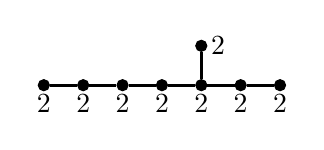
\begin{tikzpicture}
			\tikzset{dynode/.style={circle, draw, fill=black,
						minimum size=4pt, inner sep=0pt}}
			\tikzset{dyline/.style={line width=1pt}}
			\tikzset{dydash/.style={line width=1pt, dashed}}

			\begin{scope}[yshift=-10em, xshift=0]
				\node[dynode] (a1) at (0,0) {};
				\node[dynode] (a2) at (0.5,0) {};
				\node[dynode] (a3) at (1,0) {};
				\node[dynode] (a4) at (1.5,0) {};
				\node[dynode] (a5) at (2,0) {};
				\node[dynode] (a6) at (2.5,0) {};
				\node[dynode] (a7) at (3,0) {};
				\node[dynode] (a8) at (2,0.5) {};

				\draw[dyline] (a1) -- (a2) -- (a3) -- (a4) -- (a5) -- (a6) -- (a7);
				\draw[dyline] (a5) -- (a8);

				\node[below] () at (a1) {$2$};
				\node[below] () at (a2) {$2$};
				\node[below] () at (a3) {$2$};
				\node[below] () at (a4) {$2$};
				\node[below] () at (a5) {$2$};
				\node[below] () at (a6) {$2$};
				\node[below] () at (a7) {$2$};
				\node[right] () at (a8) {$2$};
			\end{scope}
		\end{tikzpicture}
		\quad\implies\quad
		\begin{pmatrix}
			2 & 1 &   &   &   &   &   &   \\
			1 & 2 & 1 &   &   &   &   &   \\
			  & 1 & 2 & 1 &   &   &   &   \\
			  &   & 1 & 2 & 1 &   &   &   \\
			  &   &   & 1 & 2 & 1 & 0 & 1 \\
			  &   &   &   & 1 & 2 & 1 & 0 \\
			  &   &   &   & 0 & 1 & 2 & 0 \\
			  &   &   &   & 1 & 0 & 0 & 2 \\
		\end{pmatrix}
	\]
	where each vertex of the tree is weighed by $2$.
\end{proposition}

It's interesting to note that if $Q$ is a matrix associated to a tree $T$, then $P(Q)$ has a $1$-skeleton homotopy equivalent to $T$. This connection between the $1$-skeleton and plumbing along a tree or graph was first noticed by Hirzebruch. It makes sense then why we'd care about matrices arising from trees instead of from general graphs which may contain cycles -- cycles break the simple-connectedness of the constructed manifold and are thereby much more complicated to work with.

% \begin{figure}[ht]\label{fig:negative-definite-trees}
% 	\centering
% 	\begin{tikzpicture}
% 		\tikzset{dynode/.style={circle, draw, fill=black,
% 					minimum size=4pt, inner sep=0pt}}
% 		\tikzset{dyline/.style={line width=1pt}}
% 		\tikzset{dydash/.style={line width=1pt, dashed}}
%
% 		\begin{scope}[yshift=0, xshift=22em]
% 			\node[dynode] (a1) at (0,0) {};
% 			\node[dynode] (a2) at (0.5,0) {};
% 			\node[dynode] (a3) at (1,0) {};
% 			\node[dynode] (a4) at (1.5,0) {};
% 			\node[dynode] (a5) at (2,0) {};
% 			\node[dynode] (a6) at (2.5,0) {};
% 			\node[dynode] (a7) at (3,0) {};
% 			\node[dynode] (a8) at (2,0.5) {};
%
% 			\draw[dyline] (a1) -- (a2) -- (a3) -- (a4) -- (a5) -- (a6) -- (a7);
% 			\draw[dyline] (a5) -- (a8);
%
% 			\node[] (l) at (1.75,-0.5) {$\E_8$};
% 		\end{scope}
%
% 		\begin{scope}[yshift=0, xshift=10em]
% 			\node[dynode] (a1) at (0,0) {};
% 			\node[dynode] (a2) at (0.5,0) {};
% 			\node[dynode] (a3) at (1,0) {};
% 			\node[dynode] (a4) at (1.5,0) {};
% 			\node[dynode] (a5) at (2,0) {};
% 			\node[dynode] (a6) at (2.5,0) {};
% 			\node[dynode] (a8) at (1.5,0.5) {};
%
% 			\draw[dyline] (a1) -- (a2) -- (a3) -- (a4) -- (a5) -- (a6);
% 			\draw[dyline] (a4) -- (a8);
%
% 			\node[] (l) at (1.5,-0.5) {$\E_7$};
% 		\end{scope}
%
% 		\begin{scope}[yshift=0, xshift=0]
% 			\node[dynode] (a1) at (0,0) {};
% 			\node[dynode] (a2) at (0.5,0) {};
% 			\node[dynode] (a3) at (1,0) {};
% 			\node[dynode] (a4) at (1.5,0) {};
% 			\node[dynode] (a5) at (2,0) {};
% 			\node[dynode] (a8) at (1,0.5) {};
%
% 			\draw[dyline] (a1) -- (a2) -- (a3) -- (a4) -- (a5);
% 			\draw[dyline] (a3) -- (a8);
%
% 			\node[] (l) at (1,-0.5) {$\E_6$};
% 		\end{scope}
%
% 		\begin{scope}[yshift=5em, xshift=3em]
% 			\node[dynode] (a1) at (0,0) {};
% 			\node[dynode] (a3) at (0.5,0) {};
% 			\node[dynode] (a4) at (1,0) {};
% 			\node[dynode] (a5) at (2.5,0) {};
% 			\node[dynode] (a6) at (3.0,0) {};
%
% 			\draw[dyline] (a1) -- (a3) -- (a4);
% 			\draw[dydash] (a4) -- (a5);
% 			\draw[dyline] (a5) -- (a6);
%
% 			\node[] (l) at (1.75,-0.5) {$\op{A}_n$};
% 		\end{scope}
%
% 		\begin{scope}[yshift=5em, xshift=17em]
% 			\node[dynode] (a1) at (0,0.4) {};
% 			\node[dynode] (a2) at (0,-0.4) {};
% 			\node[dynode] (a3) at (0.5,0) {};
% 			\node[dynode] (a4) at (1,0) {};
% 			\node[dynode] (a5) at (2.5,0) {};
% 			\node[dynode] (a6) at (3.0,0) {};
%
% 			\draw[dyline] (a1) -- (a3);
% 			\draw[dyline] (a2) -- (a3);
% 			\draw[dyline] (a3) -- (a4);
% 			\draw[dydash] (a4) -- (a5);
% 			\draw[dyline] (a5) -- (a6);
%
% 			\node[] (l) at (1.75,-0.5) {$\op{D}_n$};
% 		\end{scope}
% 	\end{tikzpicture}
% 	\vspace{1em}
% 	\caption{\todo{describe}}
% \end{figure}

\subsection{Homotopy Type of Plumbed Manifolds}



\section{Spherical Modifications}

The basic observation underlying much of surgery theory is based on the fact that for manifolds $X$ and $Y$ with boundary, we have
\[
	\partial (X\times Y) = (\partial X \times Y)\cup (X\times \partial Y).
\]
As a consequence, for integers $p,q$ the space $S^q\times S^{q-1}$ can be viewed either as the boundary of $D^{p+1}\times S^{q-1}$ or as the boundary of $S^p\times D^q$ since
\[
	\partial (S^p\times D^q) = S^p\times S^{q-1} = \partial (D^{p+1}\times S^{q-1}).
\]
Since the two products have the same boundary, whenever we find an embedding of $D^{p}\times S^{q}$ in a manifold, we can cut it out and replace it with $D^{p+1}\times S^{q-1}$.

\begin{definition}\label{def:surgery}
	Let $M$ be a smooth oriented manifold. If $f : S^q\times D^{n-q} \to M$ is a smooth embedding which maps into the interior of $M$, the \defn{surgery} of $M$ along $f$ is the smooth manifold
	\begin{equation}\label{eq:surgery-definition}
		\chi_f(M) = \left[M-\Int f(S^q\times D^{n-q})\right]\cup_{g} (D^{q+1}\times S^{n-q+1}).
	\end{equation}
	Here $g$ is the map identifying $\partial f(S^q\times D^{n-q})=f(S^q\times S^{n-q+1})$ with $\partial (D^{q+1}\times S^{n-q+1})=S^q\times S^{n-q}$.
\end{definition}

Note that $\partial (M-\Int f(S^q\times D^{n-1})) = \partial M \sqcup f(S^q\times S^{q-1})$ so $\partial \chi_f(M) = \partial M$, so surgery along an embedding into the interior does not affect the boundary.

\begin{example}\label{exam:surgery-on-a-compact-surface}
	A simple yet non-trivial example of surgery is on a surface $X_g$ of genus $g$.
	When $q=1$, note that $S^q\times D^{n-q} = S^1\times D^1$ is a cylinder, and $D^{q+1}\times S^{n-q-1}=D^2\times S^0$ is a dijsoint union of disks.
	If we embed a cylinder $S^1\times D^1$ into a ``handle'' of $X_g$, the resulting surgery cuts off this handle and reduces the genus by one. By a sequence of $g$ surgeries along embedded cylinders, we can turn $X_g$ into a sphere $X_0 = S^2$.
	\begin{figure}[ht]
		\centering
		\import{graphics/temp-diagrams/}{surgery-on-two-holed-torus.pdf_tex}
		\caption{Turning a genus 2 surface into a genus 1 surface via surgery.}\label{fig:surgery-on-two-holed-torus}
	\end{figure}
\end{example}

\begin{remark}
	Technically, the result of \cref{eq:surgery-definition} does not have an a priori smooth structure at the gluing set $f(S^q\times S^{n-q+1})$.
	\todo{smoothing out the corners.}
\end{remark}

While surgery clearly alters the topology of a manifold, it preserves the cobordism type.
\begin{definition}
	The \defn{trace}[trace of a surgery] $W_f(M)$ of a surgery $\chi_f(M)$ is the space
	\[
		W_f(M) = (D^{q+1}\times D^{n-q})\cup_h (M\times I)
	\]
	where $h$ is the map identifying $\partial D^{q+1}\times D^{n-q}$ with $f(S^q\times D^{n-q})\times \{1\}$.
\end{definition}

Note that $\partial W_f(M) = \chi_f(M) \sqcup (-M)$, so $W_f(M)$ is a cobordism $\chi_f(M) \bord M$. Consequently, surgery does not affect the cobordism type of a manifold and can thus be used to find a simplest representative for a given cobordism class.

\todo{finish this section}

\section{Framed Surgery}

\begin{definition}
	A \defn{framed manifold} is a pair $(M, F)$ consisting of a manifold $M$ and a \defn{framing}[framing of a manifold] $F$ which is a trivialization of the stable tangent bundle $\T M \oplus\underline{\R}^q$ for some $q>0$.
\end{definition}

\begin{definition}
	A \defn{framed cobordism} is
\end{definition}

\begin{theorem}
	Let $W$ be a compact framed manifold of dimension $n\geq 4$ such that the boundary $\partial W$ is a homology sphere. By a sequence of framed surgeries, $W$ can be made $\lfloor\frac{n-1}{2}\rfloor$-connected.
\end{theorem}

\begin{corollary}
	For any $k\geq 2$, we have $\bP^{2k+1}=0$.
\end{corollary}

\todo{finish this section}


\subsection{The Plumbing Theorem}\label{sec:plumbing-theorem}

\begin{proposition}
	If $\partial P^{2m}(Q)$ is a homotopy sphere then $Q$ is unimodular.
\end{proposition}

\begin{theorem}
	When $k>1$, $\partial P^{4k}(Q)$ is a homotopy sphere if and only if $Q$ is unimodular.
\end{theorem}


\begin{proposition}
	The signature of a highly-connected $4k$-dimensional manifold boundary empty or a homotopy sphere is divisible by $8$.
\end{proposition}

\begin{definition}
	For $k>1$, the \defn{Milnor sphere} is the homotopy sphere $\partial P^{4k}(E_8)$.
\end{definition}

\begin{definition}
	\todo{normal map}
\end{definition}

\begin{definition}
	\todo{surgical invariant $\sigma$}
\end{definition}

\begin{theorem}[Plumbing Theorem]\label{thm:plumbing-theorem}
	When $m>2$, there is a normal map \[(g,c) : (W,\partial W) \to (D^{2m}, S^{2m-1})\] which restricts to a homotopy equivalence $g|_{\partial W} : \partial W \to  S^{2m-1}$ with the invariant $\sigma(g,c)$ taking on any integer value.
\end{theorem}

\subsection{Surgery Theory in General}
\todo{general exact sequence}
\[
	L_{n+1}(\Z[\pi_1(X)]) \lkxto \mathcal{S}^\DIFF(X) \lkxto {[X, G/\DIFF]} \lkxto L_n(\Z[\pi_1(X)])
\]



\chapter{Geometric Invariants}\label{chap:detection}
\section{Secondary Invariants}

\section{Invariants From Integrality}

\subsection{Milnor's Invariant}

\subsection{The Eells-Kupier Invariant}

\subsection{The Witten Genus and Exotic $\mathbf{23}$-Spheres}


\chapter{Very Exotic Spheres}\label{chap:homotopy}
\section{The Thom-Pontryagin Construction}\label{sec:thom-pontryagin}

\section{The Kervaire Invariant Problem}\label{sec:kervaire-invariant-problem}

\subsection{Kervaire-Milnor Braid}\label{sec:kervaire-milnor-braid}


\begin{appendices}
	\chapter{Differential Geometry}\label{chap:differential_geometry}
	\begin{flushleft}
	\textsl{I admire the elegance of your method of computation;}\\
	\textsl{it must be nice to ride through these fields upon the}\\
  \textsl{horse of true mathematics while the like of us have to}\\
  \textsl{make our way laboriously on foot.}\\
	\rule[0pt]{24em}{0.5pt}\\
	-- \textsc{Albert Einstein} to \textsc{Tullio Levi-Civita}\\
	\vspace{2em}
\end{flushleft}

\begin{definition}\label{defn:manifold_structure}
  Let $(G,\rho)$ be an $n$-dimensional symmetry type and suppose $X$ is an $n$-dimensional manifold with frame bundle $\varpi : \B X \to X$. A \defn{$(G,\rho)$-structure} on $X$ is a reduction of $\varpi$ along the representation $\rho : G \to \GL_n$.
\end{definition}

\section{Lie Groups and Lie Algebras}

\section{Connections on Principal Bundles}


	\chapter{Explicit Constructions}\label{chap:explicit-constructions}
	\begin{flushleft}
	\textsl{}\\
	\rule[0pt]{15em}{0.5pt}\\
	\textsl{-- }
	\vspace{2em}
\end{flushleft}

\todo{introduction}

\section{The First Exotic Sphere}\label{sec:first-exotic-sphere}

We mentioned briefly in \cref{sec:plumbing} that the original constructions of $7$-dimensional exotic spheres by Milnor in \cite{milnor1956manifolds} were as total spaces of $S^{3}$ bundles over $S^4$. In this section, we'll explicitly work through this case, directly constructing a smooth manifold and proving that it is homeomorphic but not diffeomorphic to the standard $7$-dimensional sphere.

First, recall that there is an equivalence between $S^3$ bundles, $D^4$ bundles, and rank $4$ vector bundles by taking associated bundles since the linear symmetry groups of every one of $S^3\subset D^4\subset \R^4$ are isomorphic. Such bundles on $S^4$ are classified by the clutching function, which lives as an element in $\pi_3(\SO_4)$. For a review of the clutching construction, see \cref{sec:vector-bundles-over-spheres}. 
Understanding $S^3$ bundles over $S^4$ thus involves understanding the homotopy group $\pi_3(\SO_4)$. Note that there is a canonical identification of $S^3$ with the set of quaternions of unit norm, and of $\SO_4$ with rotations of the quaternionic plane $\HH$. 

\begin{proposition}
	There is an isomorphism $\Z\oplus \Z\cong \pi_3(\SO_4)$ which sends a pair $(i,j)$ to the map sending a unit quaternion $u\in S^3$ to the rotation $(v\mapsto u^i\cdot v\cdot u^j)\in \SO_4$.
\end{proposition}

\begin{proof}
	\color{red}
	\todo{this proof}

The direct approach involves viewing $\SO_4$ as the group of orientation-preserving isometries of $\R^4$, or equivalently as rotations of $S^3$. Let's consider $S^3\cong \SU_2\subset \HH$ as the set of unit norm quaternions. Letting $\SO_3$ act on the $\{i,j,k\}$ plane in $S^3$, note that any rotation $R\in \SO_4$ gives a rotation $R^{-1}(1)R\in \SO_3$ which now fixes $1$ and thus only acts on the $\{i,j,k\}$ plane. 
\begin{changemargins}
\begin{lemma}\label{prop:SO4-decomposition}
	There is a homeomorphism
	\begin{equation}
		\lkxfunc{}{\SO_4}{\SU_2\times \SO_3}{R}{\left(R(1),R^{-1}(1)R\right)}
	\end{equation}
	with inverse given by sending $(\xi, R)\in \SU_2\times \SO_3$ to the rotation $v\mapsto \xi \cdot R(v)$ where $\cdot$ denotes quaternion multiplication in $\SU_2$.
\end{lemma}
\end{changemargins}

% Next, note that 
%
% \begin{proposition}
% \end{proposition}
% \begin{proof}
% \end{proof}

Next, we recall that $\SU_2$ can be viewed as a double cover of $\SO_3$. One way to construct this double cover is by starting with the 
conjugation map $\rho : \HH \to \Aut(\HH)$ which sends $\xi$ to the automorphism $(v\mapsto \xi\cdot v\cdot \xi^{-1})$. If we restrict $\rho$ to $\SU_2\subset \HH$, the map becomes $\rho : \SU_2 \to \SO_3$. This can be shown to be a double cover by an isomorphism of $\SO_3$ with $\RP^3$. The double cover map leads to an identification of $\SU_2$ with the spin group $\Spin_3$.
\begin{proposition}
	There is an exceptional isomorphism $\Spin_3\cong \SU_2$.
\end{proposition}

It follows that $\pi_3(\SU_2)$

A bit more abstractly, we can double cover $\SO_4$ by the spin group $\Spin_4$. 
\begin{proposition}\label{prop:exceptional-isomorphism-spin4}
	There is an exceptional isomorphism $\Spin_4\cong \SU_2\times \SU_2$.
\end{proposition}
\begin{proof}
	To see that there is a hoemorphism at all, note that by \cref{prop:SO4-decomposition} we have a homeomorphism $\SO_4\cong \SU_2\times \SO_3$. Since there is an exceptional isomorphism $\Spin_3\cong \SU_2$, it follows that the double cover of $\SO_4$ would be homeomorphic to $\SU_2\times \SU_2\times \SU_2$ since this is the unique

	For a full proof that there is an isomorphism of Lie groups, see Theorem 8.1 in \cite{lawson1989spin}.
	\todo{cite spin geometry}
\end{proof}
Since covering spaces induce isomorphisms of higher homotopy groups, we have $\pi_3(\SO_4)\cong \pi_3(\Spin_4)$, and by \cref{prop:exceptional-isomorphism-spin4} we have isomorphisms 
\[\pi_3(\Spin_4)\cong \pi_3(\SU_2\times \SU_2) \cong \pi_3(S^3\times S^3)\cong \pi_3(S^3)\oplus \pi_3(S^3) = \Z\oplus \Z\]
since $\SU_2\cong S^3$. The result $\pi_3(\SO_4)\cong \Z\oplus \Z$ follows as with the direct computation, although it's trickier to see in this case that quaternion conjugation gives the representatives of homotopy classes.
\end{proof}

Let's now see which $(i,j)\in \pi_3(\SO_4)$ give us spaces homeomorphic to spheres. Let $\Sigma_{i,j}^7$ denote the total space of the $S^3$ bundle corresponding to $(i,j)$. Note that by giving $S^3$ and $S^4$ their usual smooth structures, $\Sigma_{i,j}^7$ gets a smooth structure as well. These manifolds are known as \defn{Milnor manifolds}.

\begin{proposition}
	When $i+j=1$, there is a homeomorphism $\Sigma_{i,j}^7\cong S^7$.
\end{proposition}

There are two proofs, both of which are enlightening. In the first proof, we make use of Morse theory in the form of Reeb's theorem which requires us to construct a Morse function with exactly two critical points to prove a manifold is homeomorphic to a sphere. For the second proof, we compute the homotopy type and use the topological Poincar\'e conjecture in dimension $7$.

\begin{proof}[First Proof]
	Recall that the clutching construction for $\Sigma_{i,j}^7$ is the quotient space
	\[
		\Sigma_{i,j}^7 = (D^4_+\times S^3)\cup_{h_{i,j}} (D^4_-\times S^3)
	\]
	where $h_{i,j}$ identifies $(u,v)\in\partial D^4_+ \times S^3$ with $(u, u^i\cdot v\cdot u^j)\in \partial D^4_-\times S^3$.
	Consider the function
	\[
		f : 
	\]
\end{proof}

\begin{proof}[Second Proof]
Since we have a fiber bundle
\[
		S^3 \lkxto \Sigma_{i,j}^7 \lkxto S^4,
\]
we can apply the long exact sequence of a fibration to get 
\[
	\cdots \lkxto \pi_{k+1}(S^{4}) \lkxto[\delta] \pi_k(S^{3}) \lkxto \pi_k(\Sigma_{i,j}^7) \lkxto \pi_{k}(S^{4})\lkxto[\delta] \cdots
\]
It's clear that $\Sigma_{i,j}^7$
\end{proof}




\[
	S^{n-1} \lkxto M \lkxto S^n
\]
for a manifold $M$, there is a long exact sequence of homotopy groups
\[
	\cdots \lkxto \pi_{k+1}(S^{n}) \lkxto[\delta] \pi_k(S^{n-1}) \lkxto \pi_k(M) \lkxto \pi_{k}(S^{n})\lkxto[\delta] \cdots
\]
If the connecting map $\delta : \pi_{n}(S^n) \to \pi_{n-1}(S^{n-1})$ is an isomorphism,

\todo{finish}

\begin{definition}
	% Let $\xi
	\todo{Milnor manifold}
\end{definition}

\todo{use Reeb's theorem to explicitly show that they are topological spheres}

\section{Gromoll-Meyer Exotic Sphere}

\begin{theorem}
	The Gromoll-Meyer sphere has non-negative sectional curvature.
\end{theorem}

\section{Dodecahedral Space}

\section{Exotic Spheres as Knots}

\subsection{Complex Singularities}

Let $F\in \C[z_0,z_1\ldots, z_n]$ be a non-constant polynomial in $(n+1)$-complex variables.
\begin{definition}
	The \defn{variety} of $F$ is the complex hypersurface given by the zero locus
	\[
		\V(F) = F^{-1}(0)=\left\{ z \in \C^{n+1}  F(z)=0\right\} \subset \C^{n+1}.
	\]
\end{definition}

\todo{cauchy riemann equations}

\begin{definition}
	The \defn{gradient} of a complex analytic function $F : \C^{n+1} \to \C$ is the $(n+1)$-tuple
	\[
		\nabla_F = \left(\frac{\partial F}{\partial z_0}, \frac{\partial F}{\partial z_1},\ldots, \frac{\partial F}{\partial z_n}\right).
	\]
	\todo{better definition}
\end{definition}

\begin{definition}
	A point $w\in \V(F)$ is a (complex) \defn{singularity}[complex singularity] if $\nabla_F(w)$ vanishes. A singularity is \defn{isolated}[isolated singularity] if there is a neighborhood surrounding $w$ which contains no other singularities.
\end{definition}

\begin{theorem}
	For small $\varepsilon>0$ the intersection of $\V(F)$ with $D_\varepsilon(w)$
\end{theorem}

\begin{proposition}
	Every sufficiently small sphere around an isolated singularity of $F$ intersects $\V(F)$ transversally in a smooth manifold.
\end{proposition}

\begin{definition}
	Let $w\in \V(F)$ be an isolated singularity. The \defn{link} of $F$ at $w$ is the intersection
	\[
		\L(F, w) = \V(F) \cap S^{2n+1}_\varepsilon(w) = \left\{ z\in \C^{n+1}  F(z)=0\textrm{ and } |z-w|<\varepsilon\right\}
	\]
	where $\varepsilon > 0$ is some sufficiently small real number so that $\L(F,w)$ is a smooth manifold intersecting the sphere $S^{2n+1}_\varepsilon(w)$ transversally.
\end{definition}

When the isolated singularity is clear, we write $\L(F)$.

\subsection{Brieskorn Manifolds}
The simplest examples of complex polynomials with isolated singularities are \todo{this}

\begin{definition}
	Let $(a_0,a_1,\ldots, a_n)$ be an $(n+1)$-tuple of integers greater than or equal to $2$. The \defn{Brieskorn polynomial} of the tuple $(a_0,a_1,\ldots, a_n)$ is given by
	\[
		F(z_0,z_1,\ldots, z_n) = z_0^{a_0} + z_1^{a_1} +\cdots + z_n^{a_n}.
	\]
	Correspondingly, we refer to $\V(F)$ as the \defn{Brieskorn variety} of the tuple and to the link at the origin $\L(F,0)$ origin as the \defn{Brieskorn manifold}. We'll use the notation
	\[
		\Sigma(a_0,a_1,\ldots, a_n) =\L(z_0^{a_0}+z_1^{a_1}+\cdots+z_n^{a_n}, 0)
	\]
	to refer to these Brieskorn manifolds.
\end{definition}


\begin{proposition}
	If $p,q\geq 2$, then $\Sigma(p,q)\subset S^3$ is the torus link of type $(p,q)$.
\end{proposition}

\begin{proposition}
	There is a homeomorphism $\Sigma(2,2,2)\cong \RP^3$.
\end{proposition}

\begin{proposition}
	There is a homeomorphism $\Sigma(2,3,5)\cong \mathscr{D}$.
\end{proposition}

\subsection{The Fibration Theorem}

\begin{theorem}\label{thm:fibration}
	If $F$ is a complex polynomial in $(n+1)$-variables with an isolated singularity at the origin, then there is a smooth fiber bundle map
	\[
		\lkxfunc{\phi}{S^{2n+1}_\varepsilon - \L(F)}{S^1}{z}{\arg F(z).}
	\]
\end{theorem}

For a given angle $e^{i\theta}\in S^1$, we'll denote the fiber of the bundle $\phi$ as $F_\theta = \phi^{-1}(e^{i\theta})$.

\begin{proposition}
	Each fiber $F_\theta$ is a smooth parallelizable $2n$-manifold.
\end{proposition}

\subsection{When is the link a topological sphere?}

Let's fix a polynomial $F$ in $(n+1)$ complex variables

\begin{proposition}
	If $n\neq 2$, then $\L$ is homeomorphic to the sphere $S^{2n-1}$ if and only if $\L$ has the homology of a sphere. In fact, $\L$ is a topological sphere if and only if the reduced homology $\widetilde{H}_{n-1}(\L)$ is trivial.
\end{proposition}

Let's now choose an orientation for $F_\theta$.

\begin{proposition}
	The manifold $\L$ is a homology sphere if and only if the intersection form
	\[
		\lkxfunc{Q_{F_\theta}}{\H_n(F_\theta)\times \H_n(F_\theta)}{\Z}
	\]
	has determinant $\pm 1$ -- in other words if $Q_{F_\theta}$ is unimodular.
\end{proposition}

\subsection{Kervaire Invariant}

\begin{theorem}[Brieskorn-Pham]
\end{theorem}

\begin{theorem}[Levine]
	If $n$ is odd, the Kervaire invariant is given by
	\[
		c(F_0) = \begin{cases}
			0 & \textrm{if }\Delta(-1)\equiv \pm 1\mod 8 \\
			1 & \textrm{if }\Delta(-1)\equiv \pm 3\mod 8
		\end{cases}
	\]
\end{theorem}

\begin{theorem}[Hirzebruch-Mayer] Smooth Brieskorn varieties are parallelizable.
\end{theorem}

	%
	% \chapter{Characteristic Classes}\label{chap:characteristic_classes}
	% % \section{The Chern-Weil Homomorphism}

\begin{definition}\label{defn:poincare-pair}
	Let $X$ be an $n$-dimensional manifold and $Y$ a closed submanifold. The pair $(X,Y)$ is said to be a \defn{Poincar\'e pair} if there is a fundamental class $[X, Y]\in \H_n(X,Y)$ such that the map
	\[
		\lkxfunc{}{\H^q(X,Y)}{\H_{n-q}(X)}{\omega}{\omega \frown [X, Y]}
	\]
	given by cap product with the fundamental class is an isomorphism.
\end{definition}

\begin{remark}\label{rmk:duality-integration}
In the case of de Rham cohomology, since $X$ is connected we have $\H_0(X)\cong \R$. Under this identification, the Poincar\'e duality isomorphism for top-dimensional relative cohomology classes $\omega\in \H^n(X,Y)$ can be interpreted as integration, i.e. $\omega\frown [X,Y]$ corresponds to $\int_X \omega$. 
\end{remark}

With this notion of a Poincar\'e pair, the classical statement of Poincar\'e duality is given:

\begin{theorem}[Poincar\'e Duality]\label{thm:poincare-duality}
	If $X$ is a closed manifold, then $(X,\emptyset)$ is a Poincar\'e pair.
\end{theorem}

\begin{theorem}[Poincar\'e-Lefschetz Duality]\label{thm:poincare-lefschetz-duality}
	If $X$ is a compact manifold with boundary, then $(X,\partial X)$ is a Poincar\'e pair.
\end{theorem}

\[
	\delta I = \int_X \omega + d\mathcal{A} - \int_X \omega =\int_X d\mathcal{A} =\int_{\partial X} \mathcal{A}
\]

\begin{definition*}
	A \defn{characteristic class} is a natural transformation 
	\[
		\lkxfunc{c}{\Bun_{G}}{h^\bullet}
	\]
	from the set of principal $G$-bundles
\end{definition*}

One of the fundamental topological invariants of a $2m$-manifold is its intersection form, a bilinear form which ``counts'' the number of intersections of submanifolds. We'll see this geometric interpretation in \cref{chap:construction_a}, but for now we'll stick to a more algebraic definition.

\begin{definition}\label{defn:intersection-form}
	Let $(X,Y)$ be a Poincar\'e pair where $X$ is a $2m$-manifold. The \defn{intersection form} of $(X,Y)$ is the bilinear form on $\H^{m}(X,Y)$ given by
	\[
		\lkxfunc{}{\H^{m}(X,Y)^{\times 2}}{\R}{\alpha, \beta}{(\alpha\smile\beta)[X,Y]}
	\]
	where $[X,Y]\in \H_{2m}(X,Y)$ is an orientation class.
\end{definition}
By the graded-commutativity of the cap product, when $m$ is odd this form is skew-symmetric and when $m$ is even this form is symmetric. For now, let's assume $m$ is even so that the form is symmetric bilinear. Following our conventions, we'll now write $2m=4k$. 


\section{Chern and Pontryagin Classes}

\begin{proposition}\label{prop:pontryagin_classes_of_CPn}
  The Pontryagin classes of complex projective space $\CP^n$ are
  \[
    p_k(\CP^n) = \binom{n+1}{k}\quad\textrm{for}\quad 1\leq k \leq n/2.
  \]
\end{proposition}

\section{Stiefel-Whitney Classes}\label{sec:stiefel-whitney_classes}

\section{Universal Bundles}\label{sec:universal_bundles}

\todo{"the most twisted bundle" from Bott and Tu}
\cite{milnorstasheff1974characteristic}
\cite{botttu1982differential}

\begin{theorem}\label{thm:cohomology_of_BO}
  There is a ring isomorphism
  \[
    \H^\bullet(\BO_n; \Z/2) \cong \Z/2[w_1,\ldots, w_n]
  \]
  where $w_i$ are Stiefel-Whitney classes of the universal bundle over $\BO_n$. In other words, any characteristic class for unoriented real bundles with $\Z/2$-coefficients can be expressed in terms of the Stiefel-Whitney classes.
\end{theorem}

\begin{theorem}\label{thm:cohomology_of_BSO}
  Let $\Lambda$ be an integral domain containing $1/2$. There are ring isomorphisms
  \[
      \H^\bullet(\BSO_{2m+1}; \Lambda) \cong \Lambda[p_1, \ldots, p_m]
      \quad\textrm{and}\quad
      \H^\bullet(\BSO_{2m}; \Lambda) \cong \Lambda[p_1, \ldots, p_m, e]/(e^2-p_m)
  \]
  where $p_i$ and $e$ are Pontryagin and Euler classes of the universal bundle over $\BSO_n$.
  In other words, ignoring $2$-torsion, any characterstic class for oriented real bundles can be expressed in terms of Pontryagin and Euler classes.
\end{theorem}

\section{Intersection Form}

	%
	\chapter{Miscellaneous Preliminaries}\label{chap:misc-appendix}
	\chapter{Miscellaneous Results}

\begin{proposition}\label{prop:splittings_affine}
  Let $A, B, C$ be vector spaces in a short exact sequence 
  \[
    0 \lkxto A \lkxto[f] B \lkxto[g] C\lkxto 0.
  \]
  The space of splittings of this short exact sequence is affine over $\Hom(C, A)$.
\end{proposition}
\begin{proof}
\end{proof}


\end{appendices}

\lkxrefs
\lkxindex

\end{document}
